%&preformat-disser
\RequirePackage[l2tabu,orthodox]{nag} % Раскомментировав, можно в логе получать рекомендации относительно правильного использования пакетов и предупреждения об устаревших и нерекомендуемых пакетах
% Формат А4, 14pt (ГОСТ Р 7.0.11-2011, 5.3.6)
\documentclass[a4paper,14pt,oneside,openany]{memoir}

\input{common/setup}            % общие настройки шаблона
\input{common/packages}         % Пакеты общие для диссертации и автореферата
\synopsisfalse                      % Этот документ --- не автореферат
\input{Dissertation/dispackages}    % Пакеты для диссертации
\input{Dissertation/userpackages}   % Пакеты для специфических пользовательских задач

\input{Dissertation/setup}      % Упрощённые настройки шаблона

\input{common/newnames}         % Новые переменные, для всего проекта

%%% Основные сведения %%%
\newcommand{\thesisAuthorLastName}{Курбанов}
\newcommand{\thesisAuthorOtherNames}{Эльдар Ровшанович}
\newcommand{\thesisAuthorInitials}{Э.\,Р.}
\newcommand{\thesisAuthor}             % Диссертация, ФИО автора
{%
    \texorpdfstring{% \texorpdfstring takes two arguments and uses the first for (La)TeX and the second for pdf
        \thesisAuthorLastName~\thesisAuthorOtherNames% так будет отображаться на титульном листе или в тексте, где будет использоваться переменная
    }{%
        \thesisAuthorLastName, \thesisAuthorOtherNames% эта запись для свойств pdf-файла. В таком виде, если pdf будет обработан программами для сбора библиографических сведений, будет правильно представлена фамилия.
    }
}
\newcommand{\thesisAuthorShort}        % Диссертация, ФИО автора инициалами
{\thesisAuthorInitials~\thesisAuthorLastName}
%\newcommand{\thesisUdk}                % Диссертация, УДК
%{\fixme{xxx.xxx}}
\newcommand{\thesisTitle}              % Диссертация, название
{СИСТЕМА УПРАВЛЕНИЯ И ФОРМИРОВАНИЯ ПОВЕДЕНЧЕСКОЙ СТРАТЕГИИ АВТОНОМНОГО МОБИЛЬНОГО РОБОТА НА ОСНОВЕ ВИЗУАЛЬНОГО АНАЛИЗА ОКРУЖАЮЩЕГО ПРОСТРАНСТВА}
\newcommand{\thesisSpecialtyNumber}    % Диссертация, специальность, номер
{02.04.03}
\newcommand{\thesisSpecialtyTitle}     % Диссертация, специальность, название (название взято с сайта ВАК для примера)
{Математическое обеспечение и администрирование информационных систем}
%% \newcommand{\thesisSpecialtyTwoNumber} % Диссертация, вторая специальность, номер
%% {\fixme{XX.XX.XX}}
%% \newcommand{\thesisSpecialtyTwoTitle}  % Диссертация, вторая специальность, название
%% {\fixme{Теория и~методика физического воспитания, спортивной тренировки,
%% оздоровительной и~адаптивной физической культуры}}
\newcommand{\thesisDegree}             % Диссертация, ученая степень
{магистра}
\newcommand{\thesisDegreeShort}        % Диссертация, ученая степень, краткая запись
{маг.}
\newcommand{\thesisCity}               % Диссертация, город написания диссертации
{Волгоград}
\newcommand{\thesisYear}               % Диссертация, год написания диссертации
{\the\year}
\newcommand{\thesisOrganization}       % Диссертация, организация
{Министерство науки и высшего образования Российской Федерации Федеральное государственное автономное образовательное учреждение высшего образования <<Волгоградский государственный университет>> Кафедра~\textit{Компьютерных наук и экспериментальной математики}}
\newcommand{\thesisOrganizationShort}  % Диссертация, краткое название организации для доклада
{Система управления роботом}

\newcommand{\thesisInOrganization}     % Диссертация, организация в предложном падеже: Работа выполнена в ...
{Министерстве науки и высшего образования Российской Федерации Федеральное государственном автономном образовательном учреждении высшего образования <<Волгоградский государственный университет>> Кафедры~\textit{Компьютерных наук и экспериментальной математики}}

%% \newcommand{\supervisorDead}{}           % Рисовать рамку вокруг фамилии
\newcommand{\supervisorFio}              % Научный руководитель, ФИО
{Клячин Владимир Александрович}
\newcommand{\supervisorRegalia}          % Научный руководитель, регалии
{доктор физико-математических наук,~профессор}
\newcommand{\supervisorJobPost}          % Научный руководитель, должность
{заведующий кафедрой КНЭМ}
\newcommand{\supervisorFioShort}         % Научный руководитель, ФИО
{В.\,В.~Клячин}
\newcommand{\supervisorRegaliaShort}     % Научный руководитель, регалии
{д.~ф.~-м.~н.,~проф.}
\newcommand{\supervisorJobPostShort}   % Научный руководитель, должность
{зав.~кафедрой КНЭМ}

%% \newcommand{\supervisorTwoDead}{}        % Рисовать рамку вокруг фамилии
\newcommand{\supervisorTwoFio}           % Второй научный руководитель, ФИО
{Гордеев Алексей Юрьевич}
%% \newcommand{\supervisorTwoRegalia}       % Второй научный руководитель, регалии
%% {\fixme{доктор физико-математических наук, профессор}}
\newcommand{\supervisorTwoJobPost}          % Научный руководитель, должность
{старший преподаватель кафедры КНЭМ}
\newcommand{\supervisorTwoFioShort}      % Второй научный руководитель, ФИО
{А.\,Ю.~Гордеев}
%% \newcommand{\supervisorTwoRegaliaShort}  % Второй научный руководитель, регалии
%% {\fixme{д.~ф.~-м.~н.,~проф.}}
\newcommand{\supervisorTwoJobPostShort}          % Научный руководитель, должность
{ст.~преп.,~каф.~КНЭМ}

%% \newcommand{\opponentOneFio}           % Оппонент 1, ФИО
%% {\fixme{Фамилия Имя Отчество}}
%% \newcommand{\opponentOneRegalia}       % Оппонент 1, регалии
%% {\fixme{доктор физико-математических наук, профессор}}
%% \newcommand{\opponentOneJobPlace}      % Оппонент 1, место работы
%% {\fixme{Не очень длинное название для места работы}}
%% \newcommand{\opponentOneJobPost}       % Оппонент 1, должность
%% {\fixme{старший научный сотрудник}}

%% \newcommand{\opponentTwoFio}           % Оппонент 2, ФИО
%% {\fixme{Фамилия Имя Отчество}}
%% \newcommand{\opponentTwoRegalia}       % Оппонент 2, регалии
%% {\fixme{кандидат физико-математических наук}}
%% \newcommand{\opponentTwoJobPlace}      % Оппонент 2, место работы
%% {\fixme{Основное место работы c длинным длинным длинным длинным названием}}
%% \newcommand{\opponentTwoJobPost}       % Оппонент 2, должность
%% {\fixme{старший научный сотрудник}}

%% \newcommand{\opponentThreeFio}         % Оппонент 3, ФИО
%% {\fixme{Фамилия Имя Отчество}}
%% \newcommand{\opponentThreeRegalia}     % Оппонент 3, регалии
%% {\fixme{кандидат физико-математических наук}}
%% \newcommand{\opponentThreeJobPlace}    % Оппонент 3, место работы
%% {\fixme{Основное место работы c длинным длинным длинным длинным названием}}
%% \newcommand{\opponentThreeJobPost}     % Оппонент 3, должность
%% {\fixme{старший научный сотрудник}}

%% \newcommand{\leadingOrganizationTitle} % Ведущая организация, дополнительные строки. Удалить, чтобы не отображать в автореферате
%% {\fixme{Федеральное государственное бюджетное образовательное учреждение высшего
%% профессионального образования с~длинным длинным длинным длинным названием}}

\newcommand{\defenseDate}              % Защита, дата
{16 июня 2022~г.~в~12 часов}
%% \newcommand{\defenseCouncilNumber}     % Защита, номер диссертационного совета
%% {\fixme{Д\,123.456.78}}
\newcommand{\defenseCouncilTitle}      % Защита, учреждение диссертационного совета
{Федеральное государственное автономное образовательное учреждение высшего образования <<Волгоградский государственный университет>>}
\newcommand{\defenseCouncilAddress}    % Защита, адрес учреждение диссертационного совета
{400062, Волгоградская область, г. Волгоград, просп. Университетский, д.100}
\newcommand{\defenseCouncilPhone}      % Телефон для справок
{+7~(8442)~46-02-63}

%% \newcommand{\defenseSecretaryFio}      % Секретарь диссертационного совета, ФИО
%% {\fixme{Фамилия Имя Отчество}}
%% \newcommand{\defenseSecretaryRegalia}  % Секретарь диссертационного совета, регалии
%% {\fixme{д-р~физ.-мат. наук}}            % Для сокращений есть ГОСТы, например: ГОСТ Р 7.0.12-2011 + http://base.garant.ru/179724/#block_30000

%% \newcommand{\synopsisLibrary}          % Автореферат, название библиотеки
%% {\fixme{Название библиотеки}}
%% \newcommand{\synopsisDate}             % Автореферат, дата рассылки
%% {\fixme{DD mmmmmmmm}\the\year~года}

% To avoid conflict with beamer class use \providecommand
\providecommand{\keywords}%            % Ключевые слова для метаданных PDF диссертации и автореферата
{}
             % Основные сведения
\input{common/fonts}            % Определение шрифтов (частичное)
\input{common/styles}           % Стили общие для диссертации и автореферата
\input{Dissertation/disstyles}  % Стили для диссертации
\input{Dissertation/userstyles} % Стили для специфических пользовательских задач

%%% Библиография. Выбор движка для реализации %%%
% Здесь только проверка установленного ключа. Сама настройка выбора движка
% размещена в common/setup.tex
\ifnumequal{\value{bibliosel}}{0}{%
    \input{biblio/predefined}   % Встроенная реализация с загрузкой файла через движок bibtex8
}{
    \input{biblio/biblatex}     % Реализация пакетом biblatex через движок biber
}

% Вывести информацию о выбранных опциях в лог сборки
\typeout{Selected options:}
\typeout{Draft mode: \arabic{draft}}
\typeout{Font: \arabic{fontfamily}}
\typeout{AltFont: \arabic{usealtfont}}
\typeout{Bibliography backend: \arabic{bibliosel}}
\typeout{Precompile images: \arabic{imgprecompile}}
% Вывести информацию о версиях используемых библиотек в лог сборки
\listfiles

%%% Управление компиляцией отдельных частей диссертации %%%
% Необходимо сначала иметь полностью скомпилированный документ, чтобы все
% промежуточные файлы были в наличии
% Затем, для вывода отдельных частей можно воспользоваться командой \includeonly
% Ниже примеры использования команды:
%
%\includeonly{Dissertation/title}
%\includeonly{Dissertation/contents,Dissertation/appendix,Dissertation/conclusion}
%
% Если все команды закомментированы, то документ будет выведен в PDF файл полностью

\begin{document}
%%% Переопределение именований типовых разделов
% https://tex.stackexchange.com/a/156050
\gappto\captionsrussian{\input{common/renames}\unskip} % for polyglossia and babel
\input{common/renames}

%%% Структура диссертации (ГОСТ Р 7.0.11-2011, 4)
% Команда для линии с нижним подчёркиванием, возможностью написания сверху текста на ней и текстом под ней.
\newcommand\superunderline[3]{$\underset{\text{#3}}{\text{\underline{\hspace{0.3cm}#1\hspace{#2}}}}$}

% Тоже самое, но ещё с отступом слева от текста (выравнивание по середине)
\newcommand\superunderlinec[3]{$\underset{\text{#3}}{\text{\underline{\hspace{#2}#1\hspace{#2}}}}$}

% "Прокаченные" типы колонок для LaTeX. Умеют выравнивать содержимое столбца по горизонтали и принимать фиксированный размер. Полезная вещь.
\newcolumntype{A}[1]{>{\raggedright\let\newline\\\arraybackslash\hspace{0pt}}m{#1}} % Выравнивание по левому краю.
\newcolumntype{B}[1]{>{\centering\let\newline\\\arraybackslash\hspace{0pt}}m{#1}} % Выравнивание по середине.
\newcolumntype{D}[1]{>{\raggedleft\let\newline\\\arraybackslash\hspace{0pt}}m{#1}} % Выравнивание по правому краю.

% Титульный лист (ГОСТ Р 7.0.11-2001, 5.1)
\thispagestyle{empty}
\begin{center}
\thesisOrganization
\end{center}
%
%\vspace{0pt plus1fill} %число перед fill = кратность относительно некоторого расстояния fill, кусками которого заполнены пустые места


%\vspace{0pt plus4fill} %число перед fill = кратность относительно некоторого расстояния fill, кусками которого заполнены пустые места
%\begin{center}
%{\large \thesisAuthor}
%\end{center}
%
\begin{center}
\textbf { %\MakeUppercase
\thesisTitle}

%\vspace{0pt plus1fill} %число перед fill = кратность относительно некоторого расстояния fill, кусками которого заполнены пустые места
{%\small
ВЫПУСКНАЯ КВАЛИФИКАЦИОННАЯ РАБОТА \\ (магистерская работа) \\ по направлению подготовки  \thesisSpecialtyNumber\ \thesisSpecialtyTitle \\ профиль <<Технология программирования>>
}

\ifdefined\thesisSpecialtyTwoNumber
{%\small
Специальность \thesisSpecialtyTwoNumber\ "---

<<\thesisSpecialtyTwoTitle>>
}
\fi

\vspace{0pt plus2fill} %число перед fill = кратность относительно некоторого расстояния fill, кусками которого заполнены пустые места

\hfill\begin{minipage}{0.55\textwidth}
			\textbf{ВЫПОЛНИЛ:} \\
			студент гр. МОС-161 \\
			\thesisAuthorLastName\ \thesisAuthorOtherNames \\
			\underline{\hspace{\textwidth}}
		\end{minipage}
%

\vspace{0pt plus1fill} %число перед fill = кратность относительно некоторого расстояния fill, кусками которого заполнены пустые места

\hfill\begin{minipage}{0.55\textwidth}
			\textbf{НАУЧНЫЙ РУКОВОДИТЕЛЬ:} \\
			зав. кафедрой \textit{КНЭМ} \\
			д.ф.-м.н., профессор \\
			Клячин Владимир Александрович \\
			\underline{\hspace{\textwidth}}
		\end{minipage}
%

\vspace{0pt plus1fill} %число перед fill = кратность относительно некоторого расстояния fill, кусками которого заполнены пустые места

\hfill\begin{minipage}{0.55\textwidth}
			\textbf{КОНСУЛЬТАНТ:} \\
			ст. преп. кафедры \textit{КНЭМ} \\
			Гордеев Алексей Юрьевич \\
			\underline{\hspace{\textwidth}}
		\end{minipage}
%

\vspace{0pt plus1fill} %число перед fill = кратность относительно некоторого расстояния fill, кусками которого заполнены пустые места

\hfill\begin{minipage}{0.55\textwidth}
			\textbf{РАБОТА ДОПУЩЕНА К ЗАЩИТЕ:} \\
			зав. кафедрой \textit{КНЭМ} \\
			д.ф.-м.н., профессор \\
			Клячин Владимир Александрович \\
			\underline{\hspace{\textwidth}}
		\end{minipage}
%

\vspace{0pt plus2fill} %число перед fill = кратность относительно некоторого расстояния fill, кусками которого заполнены пустые места

\hfill\begin{minipage}{0.55\textwidth}
			<<\underline{\hspace{1cm}}>> \underline{\hspace{3cm}} 2022 г. \\
			(протокол № \underline{\hspace{1cm}} заседания кафедры)
		\end{minipage}
%

\vspace{0pt plus4fill} %число перед fill = кратность относительно некоторого расстояния fill, кусками которого заполнены пустые места
\end{center}
%
{\centering\textbf{\thesisCity}\  \textbf{\thesisYear}\par}           % Титульный лист
\thispagestyle{empty}
\begin{center}
\thesisOrganization
\end{center}

\vspace{0.5cm}

\hfill\begin{minipage}{0.4\textwidth}
        УТВЕРЖДАЮ: \\
	Зав.~каф.~КНЭМ \\
	\underline{\hspace{3cm}} В.А. Клячин\\
	<<\underline{\hspace{1cm}}>>\underline{\hspace{3cm}} 2022г.
\end{minipage}

\vspace{1cm}

\begin{center}
ЗАДАНИЕ

На выполнение выпускной квалификационной работы

(магистерской работы)

Студента Курбанова Эльдара Ровшановича группы МОСм-201
\end{center}

\vspace{0.3cm}

\noindent Тема: Система управления и формирования поведенческой стратегии автономного мобильного
робота на основе визуального анализа окружающего пространства.

\noindent Цель: Создание и тестирование системы управления роботом на основе визуального анализа окружающего пространства, подбор комплектующих робота, а также сбор тренировочных данных для управляющей нейронной сети на основе обучения с подкреплением.

\noindent Основные задачи:

\begin{enumerate}
	\item Исследовать предметную область робототехники;
	\item Изучить существующие известные аналоги;
	\item На основе выданных требований разработать схему управления роботом и соответствующее ПО;
	\item Протестировать созданное изделие;
	\item Собрать тренировочные данные для нейронной сети.
\end{enumerate}	

\noindent Основные этапы:

\begin{enumerate}
	\item Изучение предметной области робототехники;
	\item Изучение поставленных к роботу требований;
	\item Подбор среды выполнения ПО;
	\item Подбор комплектующих для сбора необходимых данных и движения;
	\item Рассмотрение аналогов;
	\item Изучение фреймворка Robot Operating System;
	\item Создание схемы компоновки и электрификации оборудования;
	\item Создание робота, на котором будет проводиться разработка;
	\item Установка и настройка ПО;
	\item Реализация Robot Navigation Stack;
	\item Создание системы для отладки и тестирования робота;
	\item Тестирование созданного изделия;
	\item Сбор тренировочных данных для нейронной сети.
\end{enumerate}

\vspace{0.3cm}

\noindent Рекомендуемая литература:

\begin{enumerate}
	\item Joseph, L. Mastering ROS for Robotics Programming: Design, build, and simulate complex robots using the Robot Operating System, 2nd Edition [Текст] / L. Joseph, J. Cacace. — Packt Publishing, 2018. — 580 с. — Текст: непосредственный;
	
	\item Электронный ресурс: официальная документация ROS : сайт / Willow Garage, Inc. — URL: \url{http://wiki.ros.org/Documentation}. - Текст : электронный;
	
	\item Real-Time Loop Closure in 2D LIDAR SLAM / W. Hess [и др.] // 2016 IEEE International Conference on Robotics and Automation (ICRA). — Текст: электронный. — 2016. — С. 1271—1278. — URL: \url{https://storage.googleapis.com/pub-tools-public-publication-data/pdf/45466.pdf} (дата обр. 11.06.2022).
\end{enumerate}

\newcommand\tline[2]{$\underset{\text{#1}}{\text{\underline{\hspace{#2}}}}$}
\vspace{2cm}

Дата выдачи \underline{\hspace{4cm}} Срок исполнения \underline{\hspace{4.5cm}}

Руководитель: \tline{(подпись)}{5cm} \hspace{0.3cm} \tline{(ФИО)}{6.5cm}

\vspace{1cm}

Задание принял к исполнению \tline{(подпись)}{5cm}   % Задачи работы
\include{Dissertation/contents}        % Оглавление
\ifnumequal{\value{contnumfig}}{1}{}{\counterwithout{figure}{chapter}}
\ifnumequal{\value{contnumtab}}{1}{}{\counterwithout{table}{chapter}}
\chapter*{Введение}                         % Заголовок
\addcontentsline{toc}{chapter}{Введение}    % Добавляем его в оглавление

\newcommand{\actuality}{}
\newcommand{\progress}{}
\newcommand{\aim}{{\textbf\aimTXT}}
\newcommand{\tasks}{\textbf{\tasksTXT}}
\newcommand{\novelty}{\textbf{\noveltyTXT}}
\newcommand{\influence}{\textbf{\influenceTXT}}
\newcommand{\methods}{\textbf{\methodsTXT}}
\newcommand{\defpositions}{\textbf{\defpositionsTXT}}
\newcommand{\reliability}{\textbf{\reliabilityTXT}}
\newcommand{\probation}{\textbf{\probationTXT}}
\newcommand{\contribution}{\textbf{\contributionTXT}}
\newcommand{\publications}{\textbf{\publicationsTXT}}


{\actuality} Актуальность данной работы обусловлена всеобщей автоматизацией и <<роботизацией>> деятельности человека в условиях современной реальности~\cite{robotization}. Решение поставленной задачи позволит создать робота, умеющего исследовать разного вида помещения, распознавая опасные объекты, попавшие в его поле зрения. Это позволит не только делегировать на робота задачи по обнаружению, но и снизит риски травмирования или гибели человека в случае, когда объект представляет какую-либо угрозу здоровью.


{\progress} В настоящий момент поставленная данной работой задача формирования поведенческой стратегии и управления роботом решена не полностью. Требуются значительные улучшения на стороне нейронной сети, управляющей роботом, однако её создание и улучшение не являлись целью данной работы.


{\aim} данной работы является подготовка аппаратной части робота для корректного движения, а также сбор необходимых данных для обучения нейронной сети, которая будет управлять данным роботом.


Для~достижения поставленной цели необходимо было решить следующие {\tasks}:
\begin{enumerate}[beginpenalty=10000] % https://tex.stackexchange.com/a/476052/104425
  \item Исследовать предметную область робототехники\footnote{Робототехника не изучалась на протяжении всего курса обучения в университете.} (аппаратную и программную часть);
  \item Изучить существующие известные аналоги (в~т.\:ч зарубежные);
  \item Подобрать совместимый и недорогой программно-аппаратный комплекс, подходящий под задачи запуска нейронной сети;
  \item Протестировать работоспособность и совместимость аппаратной и программной частей.
\end{enumerate}


{\novelty}
\begin{enumerate}[beginpenalty=10000] % https://tex.stackexchange.com/a/476052/104425
  \item Впервые в России создана роботизированная платформа для работы с нейронной сетью на основе обучения с подкреплением на базе ROS и Jetson Xavier NX\footnote{Автором работы не было найдено подобной разработки в открытых источниках сети Интернет}.
\end{enumerate}

{\influence} данной работы заключается в создании мобильной программно-аппаратной платформы для автономной работы нейронной сети, реализующей поведенческую стратегию робота в заранее неизвестном замкнутом пространстве.

{\methods} При разработке данного робота использовались такие методы эмпирического исследования, как наблюдение и эксперимент, а к методам теоретического исследования - анализ, синтез и восхождение от абстрактного к конкретному.

{\defpositions}
\begin{enumerate}[beginpenalty=10000] % https://tex.stackexchange.com/a/476052/104425
  \item Если робот был запущен без ошибок, то он будет предоставлять все необходимые данные управляющей нейронной сети;
  \item Если роботу были предоставлены управляющие сигналы для движения, то он с минимальной задержкой и должен исполнить их.
\end{enumerate}

{\reliability} полученного результата работы обеспечивается соответствующими экспериментами. \ Результаты находятся в соответствии с договорённостями научного консультанта и автора данной работы.


{\probation}
Основные результаты работы докладывались~на:
Третьей международной конференции молодых учёных по обработке информации (YSIP3, 2019), глобальной технологической конференции 2020 года (GTC 2020 by NVIDIA).

{\contribution} Автор принимал активное участие не только в разработке программно-аппаратного комплекса робота, но и помогал в сборе обучающих данных для нейронной сети на базе обучения с подкреплением, которая будет управлять данным роботом.

\ifnumequal{\value{bibliosel}}{0}
{%%% Встроенная реализация с загрузкой файла через движок bibtex8. (При желании, внутри можно использовать обычные ссылки, наподобие `\cite{vakbib1,vakbib2}`).
    {\publications} Основные результаты по теме диссертации изложены
    в~XX~печатных изданиях,
    X из которых изданы в журналах, рекомендованных ВАК,
    X "--- в тезисах докладов.
}%
{%%% Реализация пакетом biblatex через движок biber
    \begin{refsection}[bl-author, bl-registered]
        % Это refsection=1.
        % Процитированные здесь работы:
        %  * подсчитываются, для автоматического составления фразы "Основные результаты ..."
        %  * попадают в авторскую библиографию, при usefootcite==0 и стиле `\insertbiblioauthor` или `\insertbiblioauthorgrouped`
        %  * нумеруются там в зависимости от порядка команд `\printbibliography` в этом разделе.
        %  * при использовании `\insertbiblioauthorgrouped`, порядок команд `\printbibliography` в нём должен быть тем же (см. biblio/biblatex.tex)
        %
        % Невидимый библиографический список для подсчёта количества публикаций:
        \printbibliography[heading=nobibheading, section=1, env=countauthorvak,          keyword=biblioauthorvak]%
        \printbibliography[heading=nobibheading, section=1, env=countauthorwos,          keyword=biblioauthorwos]%
        \printbibliography[heading=nobibheading, section=1, env=countauthorscopus,       keyword=biblioauthorscopus]%
        \printbibliography[heading=nobibheading, section=1, env=countauthorconf,         keyword=biblioauthorconf]%
        \printbibliography[heading=nobibheading, section=1, env=countauthorother,        keyword=biblioauthorother]%
        \printbibliography[heading=nobibheading, section=1, env=countregistered,         keyword=biblioregistered]%
        \printbibliography[heading=nobibheading, section=1, env=countauthorpatent,       keyword=biblioauthorpatent]%
        \printbibliography[heading=nobibheading, section=1, env=countauthorprogram,      keyword=biblioauthorprogram]%
        \printbibliography[heading=nobibheading, section=1, env=countauthor,             keyword=biblioauthor]%
        \printbibliography[heading=nobibheading, section=1, env=countauthorvakscopuswos, filter=vakscopuswos]%
        \printbibliography[heading=nobibheading, section=1, env=countauthorscopuswos,    filter=scopuswos]%
        %
        \nocite{*}%
        %
        {\publications} Основные результаты по теме работы изложены в~\arabic{citeauthor}~печатных изданиях,
        \arabic{citeauthorvak} из которых изданы в журналах, рекомендованных ВАК\sloppy%
        \ifnum \value{citeauthorscopuswos}>0%
            , \arabic{citeauthorscopuswos} "--- в~периодических научных журналах, индексируемых Web of~Science и Scopus\sloppy%
        \fi%
        \ifnum \value{citeauthorconf}>0%
            , \arabic{citeauthorconf} "--- в~тезисах докладов.
        \else%
            .
        \fi%
        \ifnum \value{citeregistered}=1%
            \ifnum \value{citeauthorpatent}=1%
                Зарегистрирован \arabic{citeauthorpatent} патент.
            \fi%
            \ifnum \value{citeauthorprogram}=1%
                Зарегистрирована \arabic{citeauthorprogram} программа для ЭВМ.
            \fi%
        \fi%
        \ifnum \value{citeregistered}>1%
            Зарегистрированы\ %
            \ifnum \value{citeauthorpatent}>0%
            \formbytotal{citeauthorpatent}{патент}{}{а}{}\sloppy%
            \ifnum \value{citeauthorprogram}=0 . \else \ и~\fi%
            \fi%
            \ifnum \value{citeauthorprogram}>0%
            \formbytotal{citeauthorprogram}{программ}{а}{ы}{} для ЭВМ.
            \fi%
        \fi%
        % К публикациям, в которых излагаются основные научные результаты диссертации на соискание учёной
        % степени, в рецензируемых изданиях приравниваются патенты на изобретения, патенты (свидетельства) на
        % полезную модель, патенты на промышленный образец, патенты на селекционные достижения, свидетельства
        % на программу для электронных вычислительных машин, базу данных, топологию интегральных микросхем,
        % зарегистрированные в установленном порядке.(в ред. Постановления Правительства РФ от 21.04.2016 N 335)
    \end{refsection}%
    \begin{refsection}[bl-author, bl-registered]
        % Это refsection=2.
        % Процитированные здесь работы:
        %  * попадают в авторскую библиографию, при usefootcite==0 и стиле `\insertbiblioauthorimportant`.
        %  * ни на что не влияют в противном случае
        \nocite{vakbib2}%vak
        \nocite{patbib1}%patent
        \nocite{progbib1}%program
        \nocite{bib1}%other
        \nocite{confbib1}%conf
    \end{refsection}%
        %
        % Всё, что вне этих двух refsection, это refsection=0,
        %  * для диссертации - это нормальные ссылки, попадающие в обычную библиографию
        %  * для автореферата:
        %     * при usefootcite==0, ссылка корректно сработает только для источника из `external.bib`. Для своих работ --- напечатает "[0]" (и даже Warning не вылезет).
        %     * при usefootcite==1, ссылка сработает нормально. В авторской библиографии будут только процитированные в refsection=0 работы.
}

При использовании пакета \verb!biblatex! будут подсчитаны все работы, добавленные
в файл \verb!biblio/author.bib!. Для правильного подсчёта работ в~различных
системах цитирования требуется использовать поля:
\begin{itemize}
        \item \texttt{authorvak} если публикация индексирована ВАК,
        \item \texttt{authorscopus} если публикация индексирована Scopus,
        \item \texttt{authorwos} если публикация индексирована Web of Science,
        \item \texttt{authorconf} для докладов конференций,
        \item \texttt{authorpatent} для патентов,
        \item \texttt{authorprogram} для зарегистрированных программ для ЭВМ,
        \item \texttt{authorother} для других публикаций.
\end{itemize}
Для подсчёта используются счётчики:
\begin{itemize}
        \item \texttt{citeauthorvak} для работ, индексируемых ВАК,
        \item \texttt{citeauthorscopus} для работ, индексируемых Scopus,
        \item \texttt{citeauthorwos} для работ, индексируемых Web of Science,
        \item \texttt{citeauthorvakscopuswos} для работ, индексируемых одной из трёх баз,
        \item \texttt{citeauthorscopuswos} для работ, индексируемых Scopus или Web of~Science,
        \item \texttt{citeauthorconf} для докладов на конференциях,
        \item \texttt{citeauthorother} для остальных работ,
        \item \texttt{citeauthorpatent} для патентов,
        \item \texttt{citeauthorprogram} для зарегистрированных программ для ЭВМ,
        \item \texttt{citeauthor} для суммарного количества работ.
\end{itemize}
% Счётчик \texttt{citeexternal} используется для подсчёта процитированных публикаций;
% \texttt{citeregistered} "--- для подсчёта суммарного количества патентов и программ для ЭВМ.

Для добавления в список публикаций автора работ, которые не были процитированы в
автореферате, требуется их~перечислить с использованием команды \verb!\nocite! в
\verb!Synopsis/content.tex!.
 % Характеристика работы по структуре во введении и в автореферате не отличается (ГОСТ Р 7.0.11, пункты 5.3.1 и 9.2.1), потому её загружаем из одного и того же внешнего файла, предварительно задав форму выделения некоторым параметрам

\textbf{Объем и структура работы.} Данная работа состоит из~введения,
\formbytotal{totalchapter}{глав}{ы}{}{},
заключения и
\formbytotal{totalappendix}{приложен}{ия}{ий}{}.
%% на случай ошибок оставляю исходный кусок на месте, закомментированным
%Полный объём диссертации составляет  \ref*{TotPages}~страницу
%с~\totalfigures{}~рисунками и~\totaltables{}~таблицами. Список литературы
%содержит \total{citenum}~наименований.
%
Полный объём диссертации составляет
\formbytotal{TotPages}{страниц}{у}{ы}{}, включая
\formbytotal{totalcount@figure}{рисун}{ок}{ка}{ков} и
\formbytotal{totalcount@table}{таблиц}{у}{ы}{}.
Список литературы содержит
\formbytotal{citenum}{наименован}{ие}{ия}{ий}.
    % Введение
\ifnumequal{\value{contnumfig}}{1}{\counterwithout{figure}{chapter}
}{\counterwithin{figure}{chapter}}
\ifnumequal{\value{contnumtab}}{1}{\counterwithout{table}{chapter}
}{\counterwithin{table}{chapter}}
\chapter{Теоретическая часть}\label{ch:ch1}

\section{Cреда выполнения}\label{sec:ch1/sec1}
Среда выполнения\footnote{(англ. execution environment, иногда «рантайм» от англ. runtime — «время выполнения»)} в информатике — вычислительное окружение, необходимое для выполнения компьютерной программы\cite{runtime}. 

К программной cреде робота предьявляются следующие требования:
\begin{enumerate}[beginpenalty=10000] % https://tex.stackexchange.com/a/476052/104425
  \item Деление на микропрограммы: должно быть чёткое разделение ответственности среди множества управляющих роботом компонентов;
  \item Единый стандарт общения между программами: это необходимо для корректного общения компонент;
  \item Синхронизация по времени: каждое сообщение, которым обмениваются микропрограммы должно сопровождаться временем его отправки чтобы у остальных компонент было понятие о времени отправки сообщения;
  \item Наличие общей среды для коммуникации: отправляющая сторона не должна иметь представление о том, куда ей отправить свои данные, а принимающая сторона о том, от кого эти данные взять;
  \item Управление данными: все приходящие данные нужно принять, все отправленные --- доставить. Слишком старые данные необходимо уничтожать чтобы не вызвать перегрузку на мобильном компьютере, которым оснащён робот.
\end{enumerate}

\section{Необходимые данные}\label{sec:ch1/sec2}

Для работы управляющей нейронной сети, которая не является частью данной работы, необходимы входные данные. К этим данным относятся:
\begin{enumerate}[beginpenalty=10000] % https://tex.stackexchange.com/a/476052/104425
  \item Текущее окружение робота в виде массива, элементами которого являются два значения: угол и расстояние до ближайшего препятствия;
  \item Изображение с видеокамеры робота для распознавания опасных объектов.
\end{enumerate}

На основе этих входных данных нейронная сеть должна предоставлять управляющий сигнал, который должен быть преобразован в команды для движения двигателей робота.

\section{Аппаратная часть робота}\label{sec:ch1/sec3}

К аппаратной части робота предьявляются следующие требования:
\begin{enumerate}[beginpenalty=10000] % https://tex.stackexchange.com/a/476052/104425
  \item Шасси должно быть как можно более мобильным, компактным и способно самостоятельно передвигаться;
  \item Вычисления должны проходить автономно на компьютере NVIDIA Jetson Xavier NX;
  \item Робот должен быть оснащён сканером окружающего пространства и уметь обнаруживать препятствия на любой стороне платформы;
  \item Видеокамера должна находиться по центру в передней части робота и иметь разрешение изображения не менее 720x720 пикселей.
  \item Компоненты не должны иметь высокую рыночную стоимость в следствии финансовых ограничений на данную работу.
\end{enumerate}

\section{NVIDIA Jetson Xavier NX}
Для разработки робота учебным учреждением был выделен одноплатный компьютер NVIDIA Jetson Xavier NX, изображённый на Рисунке~\cref{fig:xavier}~\cite{xavier}.

\begin{figure}[ht]
    \centerfloat{
        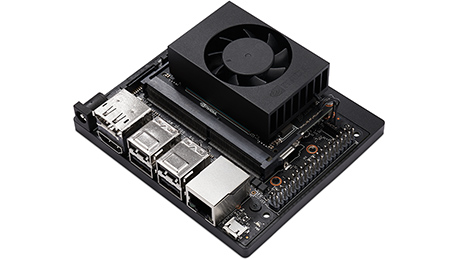
\includegraphics[scale=0.7]{xavier}
    }
    \caption{Внешний вид компьютера NVIDIA Jetson Xavier NX}\label{fig:xavier}
\end{figure}

Данный компьютер обладает следующими важными характеристиками~\cite{xavier}:

\begin{enumerate}[beginpenalty=10000] % https://tex.stackexchange.com/a/476052/104425
  \item GPU NVIDIA Volta™ с 384 ядрами CUDA и 48 тензорными ядрами;
  \item Шестиядерный 64-разрядный процессор NVIDIA Carmel с архитектурой ARM®v8.2;
  \item Оперативная память размером 8 ГБ типа LPDDR4x;
  \item Регулируемое энергопотребление: 10, 15 и 20 Вт;
  \item Интерфейс для подключения 2 CSI камер;
  \item 4 USB разъёма версии 3.0;
  \item Разъём GPIO с возможностью подключать устройства I2C;
  \item Размер платы составляет 103x90.5x31 мм.
\end{enumerate}

\FloatBarrier
           % Глава 1
\chapter{Анализ}\label{ch:ch2}

\section{Среда выполнения}\label{sec:ch2/sec1}

Проанализировав требования к среде выполнения, были представлены следующие варианты реализации:
\begin{enumerate}[beginpenalty=10000] % https://tex.stackexchange.com/a/476052/104425
  \item Собственная реализация среды на основе микросервисной клиент-серверной архитектуры;
  \item Использование стороннего фреймворка Robot Operating System (ROS).
\end{enumerate}

\subsection{Собственная реализация}
В качестве вариант рассматривалась собственная реализация среды выполнения на основе микросервисной архитектуры, включающая в себя следующее: 
\begin{enumerate}[beginpenalty=10000] % https://tex.stackexchange.com/a/476052/104425
  \item Сервер - хранилище сообщений от микросервисов. В его обязанности будут входить: приём, передача, согласование формата сообщений, удаление устаревших данных.
  \item Сами микросервисы. Помимо их основной работы, они должны принимать с сервера входные данные и отправлять выходные данные для последующей работы остальных сервисов.
\end{enumerate}

Схема представленного варианта изображена на Рисунке~\cref{fig:microservice}.

\begin{figure}[ht]
    \centerfloat{
        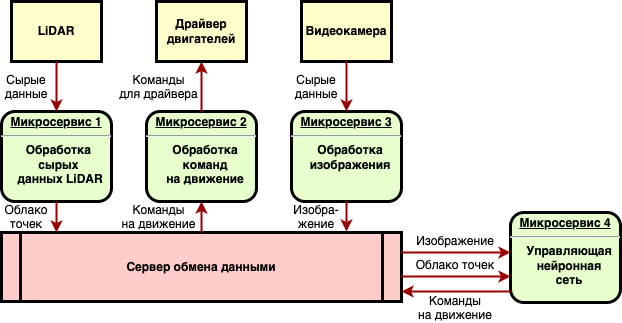
\includegraphics[scale=0.7]{microservice}
    }
    \caption{Пример архитектуры собственной реализации среды выполнения для робота на основе микросервисной архитектуры}\label{fig:microservice}
\end{figure}

Данный вариант был отвергнут в следствии существования более быстрого и удобного варианта реализации, описанного в следующей секции.

\subsection{Фреймворк Robot Operating System}
Robot Operating System или сокращённо ROS предоставляет удобные и мощные функции, помогающие разработчикам в таких задачах, как передача сообщений различного типа, распределение вычислений между компьютерами, повторное использование кода и реализация современных алгоритмов для роботов~\cite[с.~7]{ros}. В общем случае, ROS представляет собой инструмент, позволяющий связывать несколько независимых программных модулей при
помощи сервисов и узлов, которые могут передавать друг другу сообщения в различном формате. Структура ROS представлена на Рисунке~\cref{fig:ros-struct}~\cite[с.~19]{ros}.

\begin{figure}[ht]
    \centerfloat{
        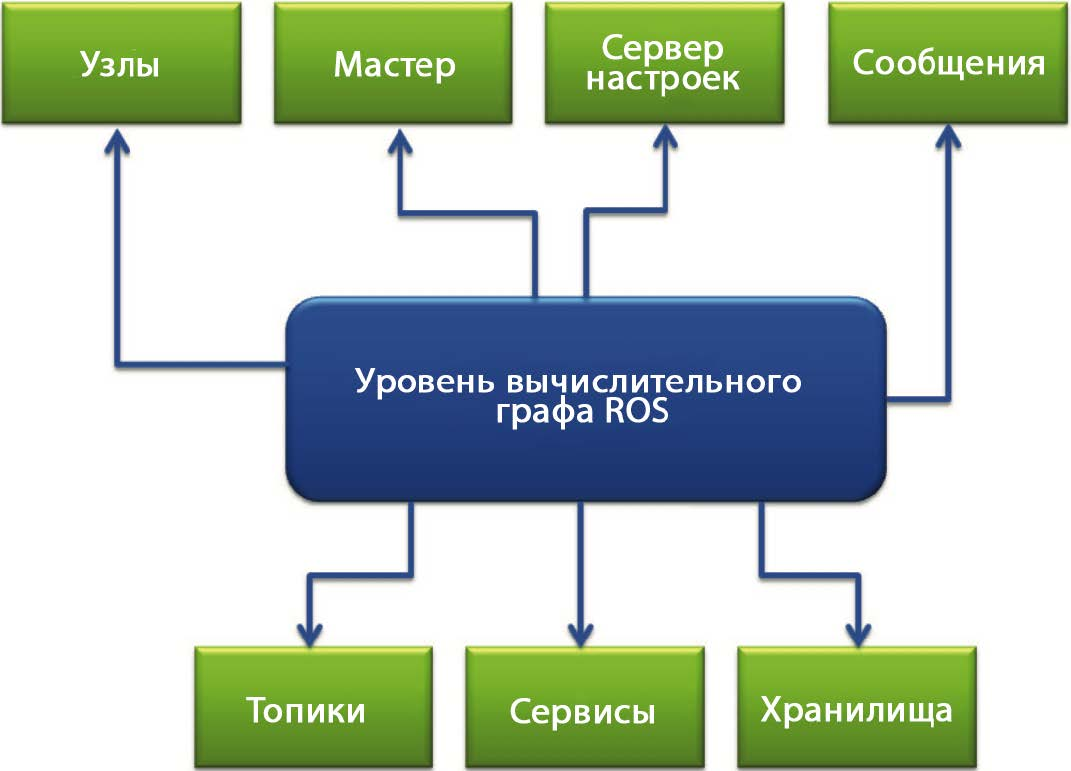
\includegraphics[scale=0.9]{ros-struct}
    }
    \caption{Общая структура Robot Operating System}\label{fig:ros-struct}
\end{figure}

Большими преимуществами использования данного фреймворка является возможность передачи сообщений по локальной сети и обширная библиотека уже реализованного ПО, которое можно без относительно больших затрат по времени интегрировать в свой собственный проект. На момент написания данной работы глобальный репозиторий ROS Index насчитывает 2455 подключенных к нему сторонних репозиториев и 6927 пакетов. Диаграмму соответствия пакетов в репозитории с версиями ROS\footnote{Версия, используемая в данной работе - ROS Melodic} можно увидеть на Рисунке~\cref{fig:ros-repo}~\cite{ros-repo}.

\begin{figure}[ht]
    \centerfloat{
        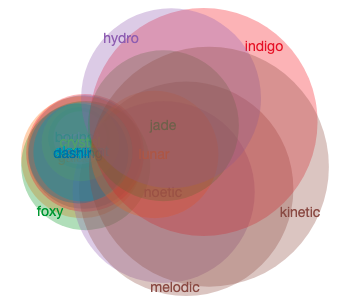
\includegraphics[scale=0.7]{ros-repo}
    }
    \caption{Диаграмма соответствия глобального репозитория ROS Index и версий ROS}\label{fig:ros-repo}
\end{figure}

\subsubsection{Концепции ROS}
Ниже приведён список концепций рассматриваемого фреймворка:

\begin{itemize}[beginpenalty=10000] % https://tex.stackexchange.com/a/476052/104425
  \item \textbf{Узел} --- это процесс, выполняющий вычисления. Каждый узел написание с использованием клиентских библиотек ROS. Используя методы связи, узлы могут общаться друг с другом заранее определённым форматом сообщений и обмениваться данными. Для этого создаются узлы-подписчики, и узлы-публикаторы;
  \item \textbf{Мастер} --- обеспечивает регистрацию и работоспособность запущенных узлов;
  \item \textbf{Сообщение} --- простая структура данных, содержащая типизированное поле, которое может содержать целый набор данных, отправляемых на другой узел. Помимо стандартных типов сообщений\footnote{Такие как целые числа, с плавающей точкой, логический тип, строковый...} возможна отправка заранее обозначенных собственных типов сообщений;
  \item \textbf{Топик} --- именованная шина данных, используемая узлами для отправки сообщений. Публикующий и подписанный узел не знают о существовании друга друга. Благодаря тому, что каждый топик имеет уникальное имя, любой узел может получить доступ к данному топику и отправляет через него данные, при условии соблюдении заранее оговорённых передаваемых типов, данным топиком;
  \item \textbf{Сервисы} --- реализация удалённого вызова процедур\footnote{RPC} в ROS. В некоторых случаях модель связи публикации и подписки может не
подходить. В этих случаях и применяют взаимодействия в виде сервисов (схема запрос/ответ), при котором один узел может запросить выполнение процедуры для другого узла, ожидая какого-то обязательного ответа\footnote{В случае использования схемы с подписчиками и публикаторами доставка сообщений и ответ
не гарантируются}~\cite[с.~20]{ros}.
\end{itemize}

\section{Обеспечение необходимых данных}
\subsection{Информация об окружающем пространстве}
Для предоставления информации об окружающем пространстве в режиме реального времени со всех сторон робота было принято решение об установке прибора лазерного сканирования, реализующего технологию LiDAR. Такое устройство представляет собой дальномер оптического диапазона, который замеряет угол и расстояние до точки, получая таким образом полярные координаты.

Существует два основных типа LiDAR'ов:

\begin{enumerate}[beginpenalty=10000] % https://tex.stackexchange.com/a/476052/104425
  \item 3D LiDAR;
  \item 2D LiDAR.
\end{enumerate}

Первый позволяет получить 3D картинку. Обычно такой LiDAR оснащён подвижным лазером, который довольно долго сканирует перед собой окружающую местность. Однако, уже сейчас можно найти 3D LiDAR, которые сканируют с довольно быстрой скоростью~\cite[с. 308]{lidar-3d}. Примером результата такой работы может стать картинка, изображённая на Рисунке~\cref{fig:lidar-3d}. На сегодняшний день такие LiDAR'ы являются довольно дорогими устройствами.

\begin{figure}[ht]
    \centerfloat{
        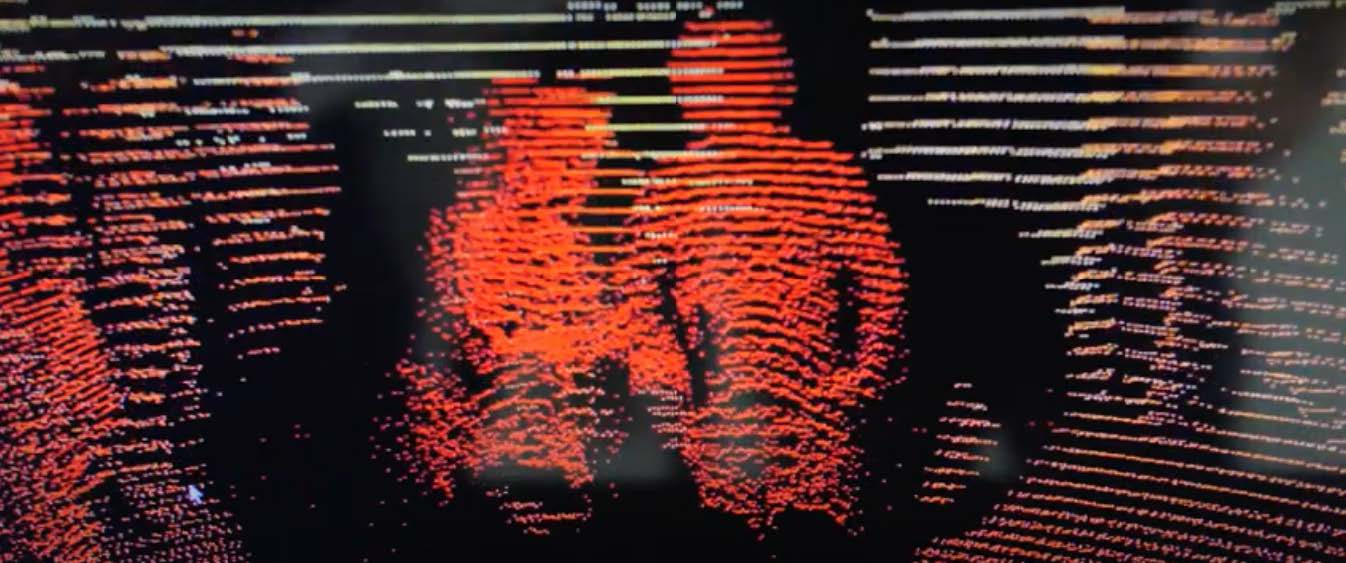
\includegraphics[scale=1.0]{lidar-3d}
    }
    \caption{Пример визуализации данных 3D LiDAR'а, представленном на выставке CEATEC 2017 компанией Panasonic Японии}\label{fig:lidar-3d}
\end{figure}

Второй, соответственно, создаёт двухмерное облако точек, которое также можно визуализировать в виде картинки, пример которой изображён на Рисунке~\cref{fig:lidar-2d}. Такой LiDAR обычно сканирует область вокруг себя и имеет угол обзора 360 градусов. Лазер также является подвижным, но только в этот раз он просто движется вокруг своей оси~\cite[с. 610]{lidar-2d}.

\begin{figure}[ht]
    \centerfloat{
        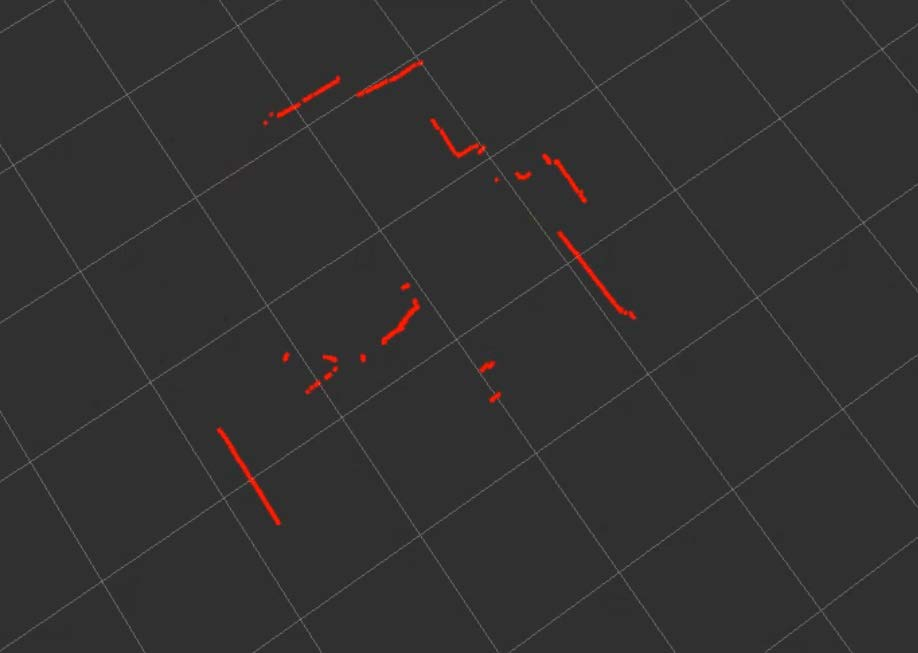
\includegraphics[scale=1.0]{lidar-2d}
    }
    \caption{Пример визуализации данных 2D LiDAR'а YDLiDAR X4}\label{fig:lidar-2d}
\end{figure}

\subsection{Альтернатива LiDAR}
В качестве альтернативы, предложенной в предыдущем пункте, можно рассмотреть иной способ получения информации об окружающем пространстве - использование камеры глубины. Одними из самых известных представителей являются камеры Xbox 360 Kinect, а также Intel RealSense Depth Camera D455, изображённые на Рисунке~\cref{fig:lidar-alts}~\cite{realsense,kinect-picture}.

\begin{figure}[ht]
    \centerfloat{
        \hfill
        \subcaptionbox[Intel® RealSense™ Depth Camera D455]{Внешний вид Intel® RealSense™ Depth Camera D455\label{fig:realsense}}{%
            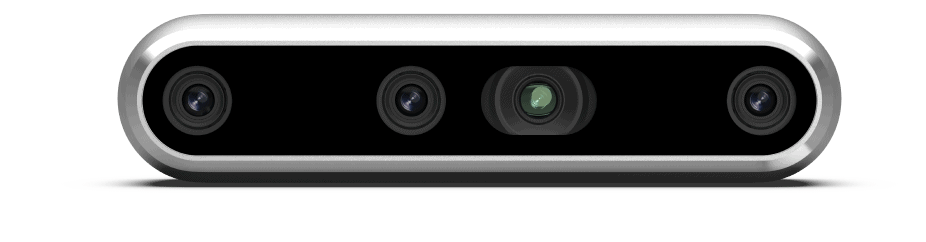
\includegraphics[width=0.5\linewidth]{realsense}}
        \hfill
        \subcaptionbox[Xbox 360 Kinect]{Внешний вид Xbox 360 Kinect\label{fig:kinect}}{%
            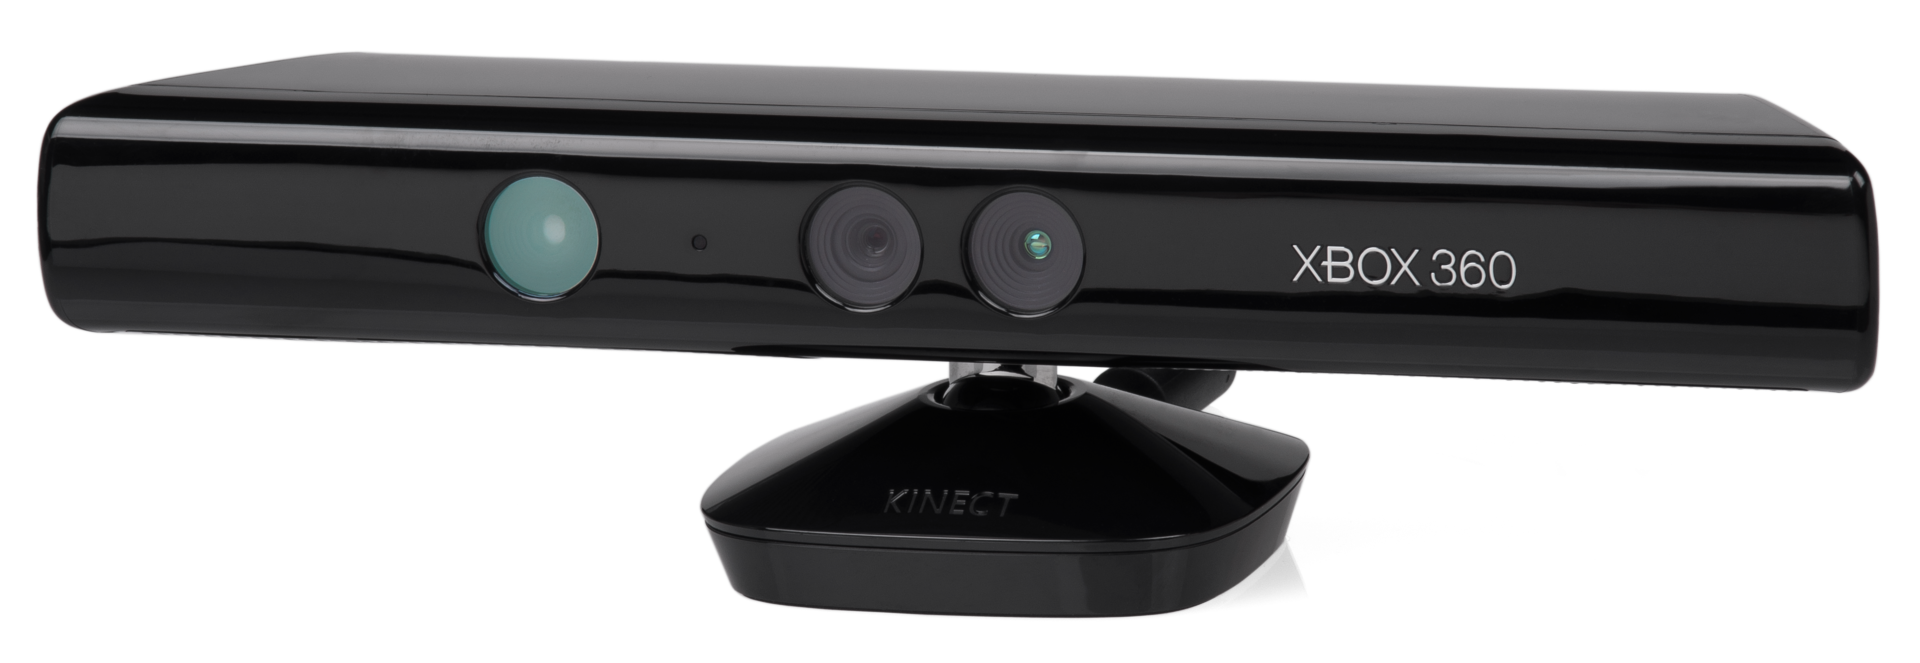
\includegraphics[width=0.5\linewidth]{kinect}}
        \hfill
    }
    \legend{}
    \caption[Камеры глубины]{Одни из самых известных камер глубины на рынке}\label{fig:lidar-alts}
\end{figure}

Камеры глубины в отличии от привычных видеокамер могут соотносить пиксели не только с цветом, но и с расстоянием до объекта в этой точке, как это показано на Рисунке~\cref{fig:depth-example}~\cite{depth-cameras}. К сожалению, данный способ получения информации об окружающем пространстве не позволит получать полную картину вокруг робота в следствии маленького угла обзора представленных камер сравнительно с лазерным сканером из предыдущего пункта данной работы.

\begin{figure}[ht]
    \centerfloat{
        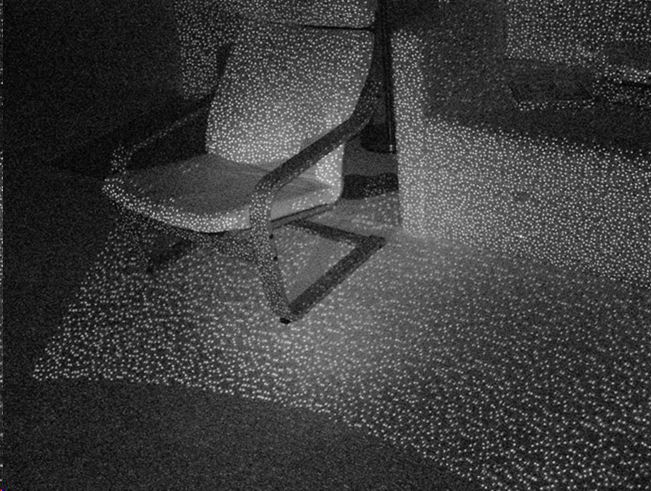
\includegraphics[scale=0.5]{depth-example}
    }
    \caption{Пример изображения с камеры глубины Xbox 360 Kinect.}\label{fig:depth-example}
\end{figure}

\subsection{Изображение с видеокамеры}
На компьютере NVIDIA Jetson Xavier NX, на котором будет работать нейросеть, существует два варианта подключения видеокамеры, которые будут рассмотрены в пунктах ниже.

\subsubsection{USB подключение}

Такой вариант подключения является самым популярным и без проблемным, так как на рынке имеется большое количество универсальных видеокамер с подключением по USB для любых целей. Для задач данной работы отлично подойдёт видеокамера Logitech C720 с разрешением видеосъёмки 1280x720 пикселей, изображённая на Рисунке~\cref{fig:usb-camera}~\cite{usb-camera}.

\begin{figure}[ht]
    \centerfloat{
        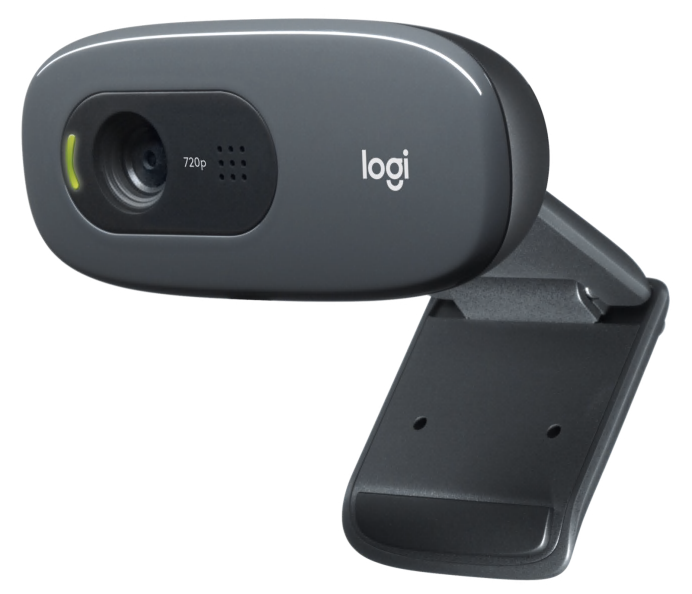
\includegraphics[scale=0.27]{usb-camera}
    }
    \caption{Внешний вид USB видеокамеры Logitech C720}\label{fig:usb-camera}
\end{figure}

\subsubsection{CSI подключение}

Данный способ подключения обладает как преимуществами, так и недостатками в сравнении с классическим USB подключением. Сравнительный анализ можно найти в Таблице~\cref{fig:usb-camera}~\cite{compare-csi-usb}.

\begin{table} [htbp]
    \centering
    \begin{threeparttable}% выравнивание подписи по границам таблицы
        \caption{Сравнение способов подключения видеокамеры к компьютеру NVIDIA Jetson Xavier NX}\label{tab:CameraCompare}%
        \begin{tabular}{| p{4cm} || p{6cm} | p{6cm}l |}
            \hline
            Рассматриваемый аспект       & \centering USB 3.0 подключение                                                 & \centering CSI подключение                                                     & \\
            \hline
            Доступность                              & \centering  Широкий выбор модельного ряда                             & \centering Единственная совместимая камера                     & \\
            \hline
            Ширина канала данных           & \centering  400 МБ/с                                                                       & \centering  320 МБ/с по одной линии (всего 4 линии)           & \\
            \hline
            Надёжность                              & \centering  USB порт, который относительно тяжело сломать & \centering Легко переламывающийся шлейф и коннектор & \\
            \hline
            Максимальная длина кабеля & \centering  Менее 5 метров                                                            & \centering  Менее 30 сантиметров                                          & \\
            \hline
            <<Горячее>> подключение    & \centering  Поддерживается                                                          & \centering  Не поддерживается                                              & \\
            \hline
            Габариты устройства              & \centering  Как правило, небольшие: 73x32x66 мм                      & \centering  Крошечный размер: 25x24x9 мм                          & \\
            \hline
        \end{tabular}
    \end{threeparttable}
\end{table}

Компьютер NVIDIA Jetson Xavier NX обладает совместимостью с единственной CSI камерой модели Sony IMX219, изображённая на Рисунке~\cref{fig:usb-camera}. Она оснащена 8 мегапиксельной матрицей с фокусным расстоянием 33 мм, а также имеет режим видеосъёмки в разрешении 1920x1080 пикселей с частотой кадров 30\footnote{1080p 30fps}~\cite{csi-camera}.

\begin{figure}[ht]
    \centerfloat{
        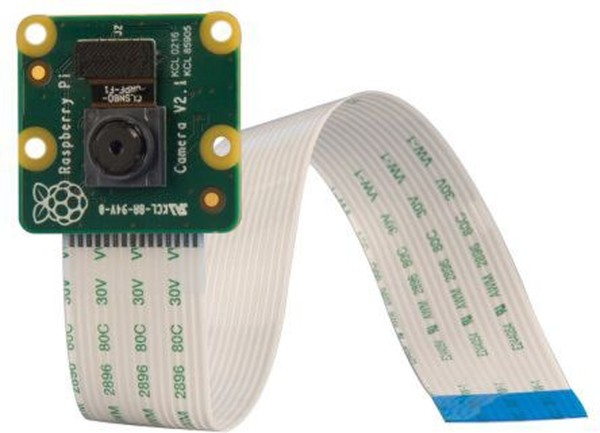
\includegraphics[scale=1.3]{csi-camera}
    }
    \caption{Внешний вид CSI видеокамеры Sony IMX219}\label{fig:csi-camera}
\end{figure}

По итогу сравнения, приоритет был дан на CSI подключение для ускорения обработки изображения, так как ресурсы мобильного компьютера сильно ограничены.

\section{Шасси робота}
Шасси робота определяет его <<мобильность>> и способность преодолевать различные препятствия. При выборе шасси необходимо искать компромиссы. С одной стороны, оно не должно быть большим, чтобы была возможность проезда в узких местах и не должно быть маленьким чтобы уместить всё оборудование на безопасном расстоянии друг от друга. 

В основной своей массе, по своей подвижной части шасси подразделяются на гусеничные и колёсные. Для робота было выбрано гусеничное шасси TS100, изображённое на Рисунке~\cref{fig:chassis}~\cite{chassis}. Такой выбор сделан чтобы отработать движения на гусеницах, которые более устойчивы к неровной поверхности дороги\footnote{В будущем предполагается использование робота в полевых условиях}.

\begin{figure}[ht]
    \centerfloat{
        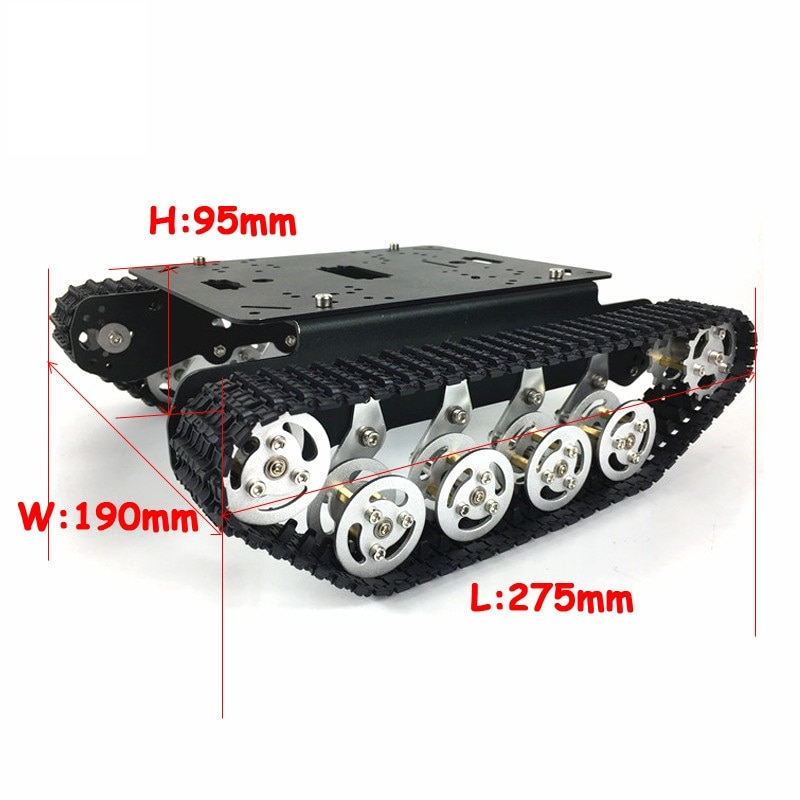
\includegraphics[scale=0.4]{chassis}
    }
    \caption{Внешний вид выбранного гусеничного шасси для робота TS100}\label{fig:chassis}
\end{figure}

Данное шасси имеет следующие характеристики~\cite{chassis}:
\begin{enumerate}[beginpenalty=10000] % https://tex.stackexchange.com/a/476052/104425
  \item Материал: алюминиевый сплав;
  \item Размер: 275x190x95 мм;
  \item Вес: 1100г.
\end{enumerate}

Шасси дополнительно укомплектовано двумя экземплярами электродвигателя DT25-370, которое изображено на Рисунке~\cref{fig:motor}~\cite{motor}.

\begin{figure}[ht]
    \centerfloat{
        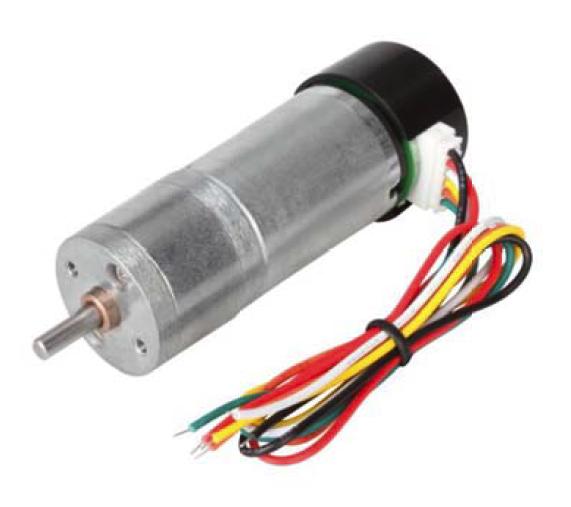
\includegraphics[scale=0.27]{motor}
    }
    \caption{Внешний вид электродвигателя DT25-370}\label{fig:motor}
\end{figure}

Двигатель имеет следующие характеристики~\cite{motor}:
\begin{enumerate}[beginpenalty=10000] % https://tex.stackexchange.com/a/476052/104425
  \item Максимальная скорость: 150 оборотов в минуту;
  \item Допустимая нагрузка: 3 кг;
  \item Рабочее напряжение: 9 вольт;
  \item Датчики Холла: 2 шт;
  \item Максимальное потребление тока: 4.5 А.
\end{enumerate}

\section{Рассмотрение аналогов}
К известным аналогам разрабатываемого робота, созданных на базе такой же платформы Jetson можно причислить роботов от самой компании NVIDIA: JetBot и Kaya. Оба эти робота были созданы для демонстрации возможностей одноплатного компьютера NVIDIA Jetson Nano.

\subsection{NVIDIA Kaya}
Данная модель компактного мобильного автономного робота была представлена на технологической конференции GTC 2019 и в первую очередь предназначается для работы с программным обеспечением Isaac SDK. Робот представлен на Рисунке~\cref{fig:kaya}.

\begin{figure}[ht]
    \centerfloat{
        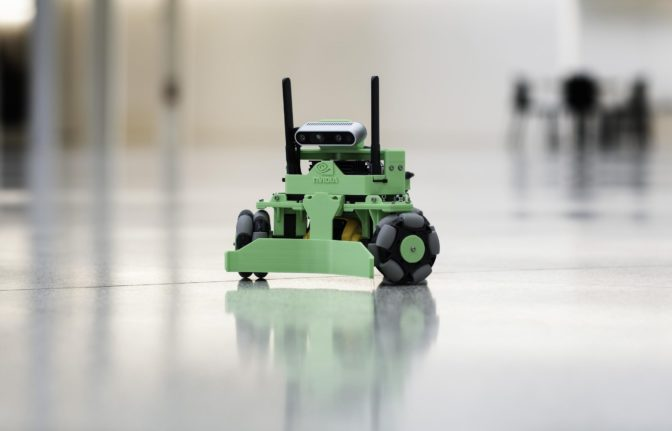
\includegraphics[scale=1.0]{kaya}
    }
    \caption{Внешний вид робота NVIDIA Kaya}\label{fig:kaya}
\end{figure}

Аппаратно данный робот помимо самого Jetson NANO включает в себя пластиковый корпус на трёх колёсах (печатаемый на 3D принтере), 3D камеру LiDAR Intel Real Sense и систему управления. Общая стоимость аппаратной части на момент написания данной работы\footnote{июнь 2022} составляет 812.87\$~\cite{kaya}.

На компьютер Jetson NANO помимо ОС Ubuntu 18.04 LTS устанавливается ПО Isaac SDK и Isaac SIM. Isaac SDK - это открытая платформа NVIDIA для интеллектуальных роботов. Она предоставляет большой набор мощных алгоритмов, базирующихся на GPU вычислениях\footnote{вычисления на видеокарте} для навигации и управления.

На данном роботе можно запускать различные готовые примеры такие как ручное управление с игрового контроллера Playstation 4, автономное следование
за AprilTag, распознавание объектов на нейронной сети DetectNetv2 и алгоритм SLAM (основан на GMapping)~\cite{isaac-kaya}.

\subsection{NVIDIA JetBot}

JetBot был представлен на той же конференции, что NVIDIA Kaya и является гораздо более доступным вариантом (цена 422.99\$ на момент написания работы) для создания DIY робота (также он в отличии от Kaya имеется в розничной продаже одним комплектом и его не нужно собирать по частям из разных магазинов). NVIDIA JetBot изображён на Рисунке~\cref{fig:jetbot}~\cite{jetbot}.

\begin{figure}[ht]
    \centerfloat{
        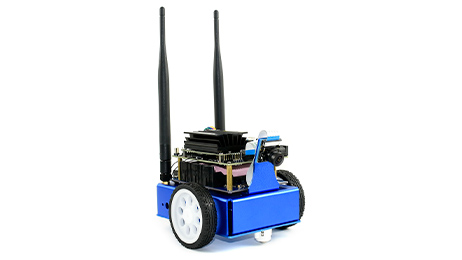
\includegraphics[scale=1.0]{jetbot}
    }
    \caption{Внешний вид робота NVIDIA JetBot}\label{fig:jetbot}
\end{figure}

Аппаратно он состоит из всё той же Nvidia Jetson Nano, двух электромоторов с драйвером в комплекте и CSI видеокамеры Sony IMX219. 

Программная часть поставляется готовым образом на базе Ubuntu 18.04 в формате ISO для прошивки MicroSD карты.

Из доступных примеров имеется простое ручное управление через кнопки на экране с возможностью прямой трансляции изображения видеокамеры на экран в браузере и автономное движение по поверхности с распознанием препятствий и пропастей в окружающем пространстве при помощи нейронной сети на основе получаемого видеосигнала. Также имеется функция следования робота за определённым целевым объектом~\cite{jetbot-examples}.

\FloatBarrier
           % Глава 2
\chapter{Практическая часть}\label{ch:ch3}

\section{Система навигации робота}\label{sec:ch3/sect1}
Исходя из требований и выбранной среды выполнения, необходимо подготовить систему навигации робота, которая будет исполнять приказы нейронной сети с максимально возможной точностью и быстродействием. Для успешной навигации понадобится:
\begin{enumerate}[beginpenalty=10000] % https://tex.stackexchange.com/a/476052/104425
  \item Возможность регулирования скорости и направления движения для всех двух двигателей робота;
  \item Некоторая метрика, определяющая реальное пройденное роботом расстояние;
  \item Интеграция данной системы с Robot Operating System.
\end{enumerate}

\subsection{ROS Navigation Stack}
В ROS уже есть готовые реализации систем навигации, которые большинстве своём универсальны и подойдут для большого количества нужд. Эта система навигации состоит из следующих компонентов:

TODO тут наумничать про ROS Navigation Stack

Для реализации данной системы необходимо подготовить инструментарий, этому посвящён следующий пункт.

\subsection{Дополнения к роботу для реализации ROS Navigation Stack}
В главе~\cref{ch:ch2} были описаны необходимые инструменты для функционирования нейронной сети, но этого недостаточно для запуска ROS Navigation Stack. Дополнительно понадобится возможность регулирования оборотов двигателей посредством использования интерфейсов, предоставляемых компьютером NVIDIA Jetson Xavier NX, а также подсчёт расстояния, пройденного роботом. 

Для регулирования оборотов двигателя было решено использовать устройство, которое называют драйвером двигателя. Его суть заключается в преобразовании цифровой команды на движение в конкретный электрический сигнал для двигателя. По сути драйвер будет являться посредником между компьютером и двигателями. К драйверу предъявляются следующие требования:

\begin{enumerate}[beginpenalty=10000] % https://tex.stackexchange.com/a/476052/104425
  \item Интерфейс управления должен быть совместим с компьютером;
  \item Устройство должно иметь маленькие габариты для установки на мобильного робота;
  \item Схема драйвера должна иметь совместимость с двигателями, установленных на шасси.
\end{enumerate}

\subsubsection{Одометрия}
Для подсчёта расстояния, пройденного роботом использована одометрия. TODO скопировать про одометрию из преддипломки

Реализация одометрии на данном роботе возможна при помощи встроенных в двигатели робота датчики Холла. TODO вставить информацию про датчики Холла

Подключение датчиков Холла было выполнено во встроенный в компьютер NVIDIA Jetson Xavier NX разъём GPIO с настройкой на приём входных данных на определённых ножках разъёма. Это подключение можно увидеть на Рисунке~\cref{fig:gpio-wire}.

\begin{figure}[ht]
    \centerfloat{
        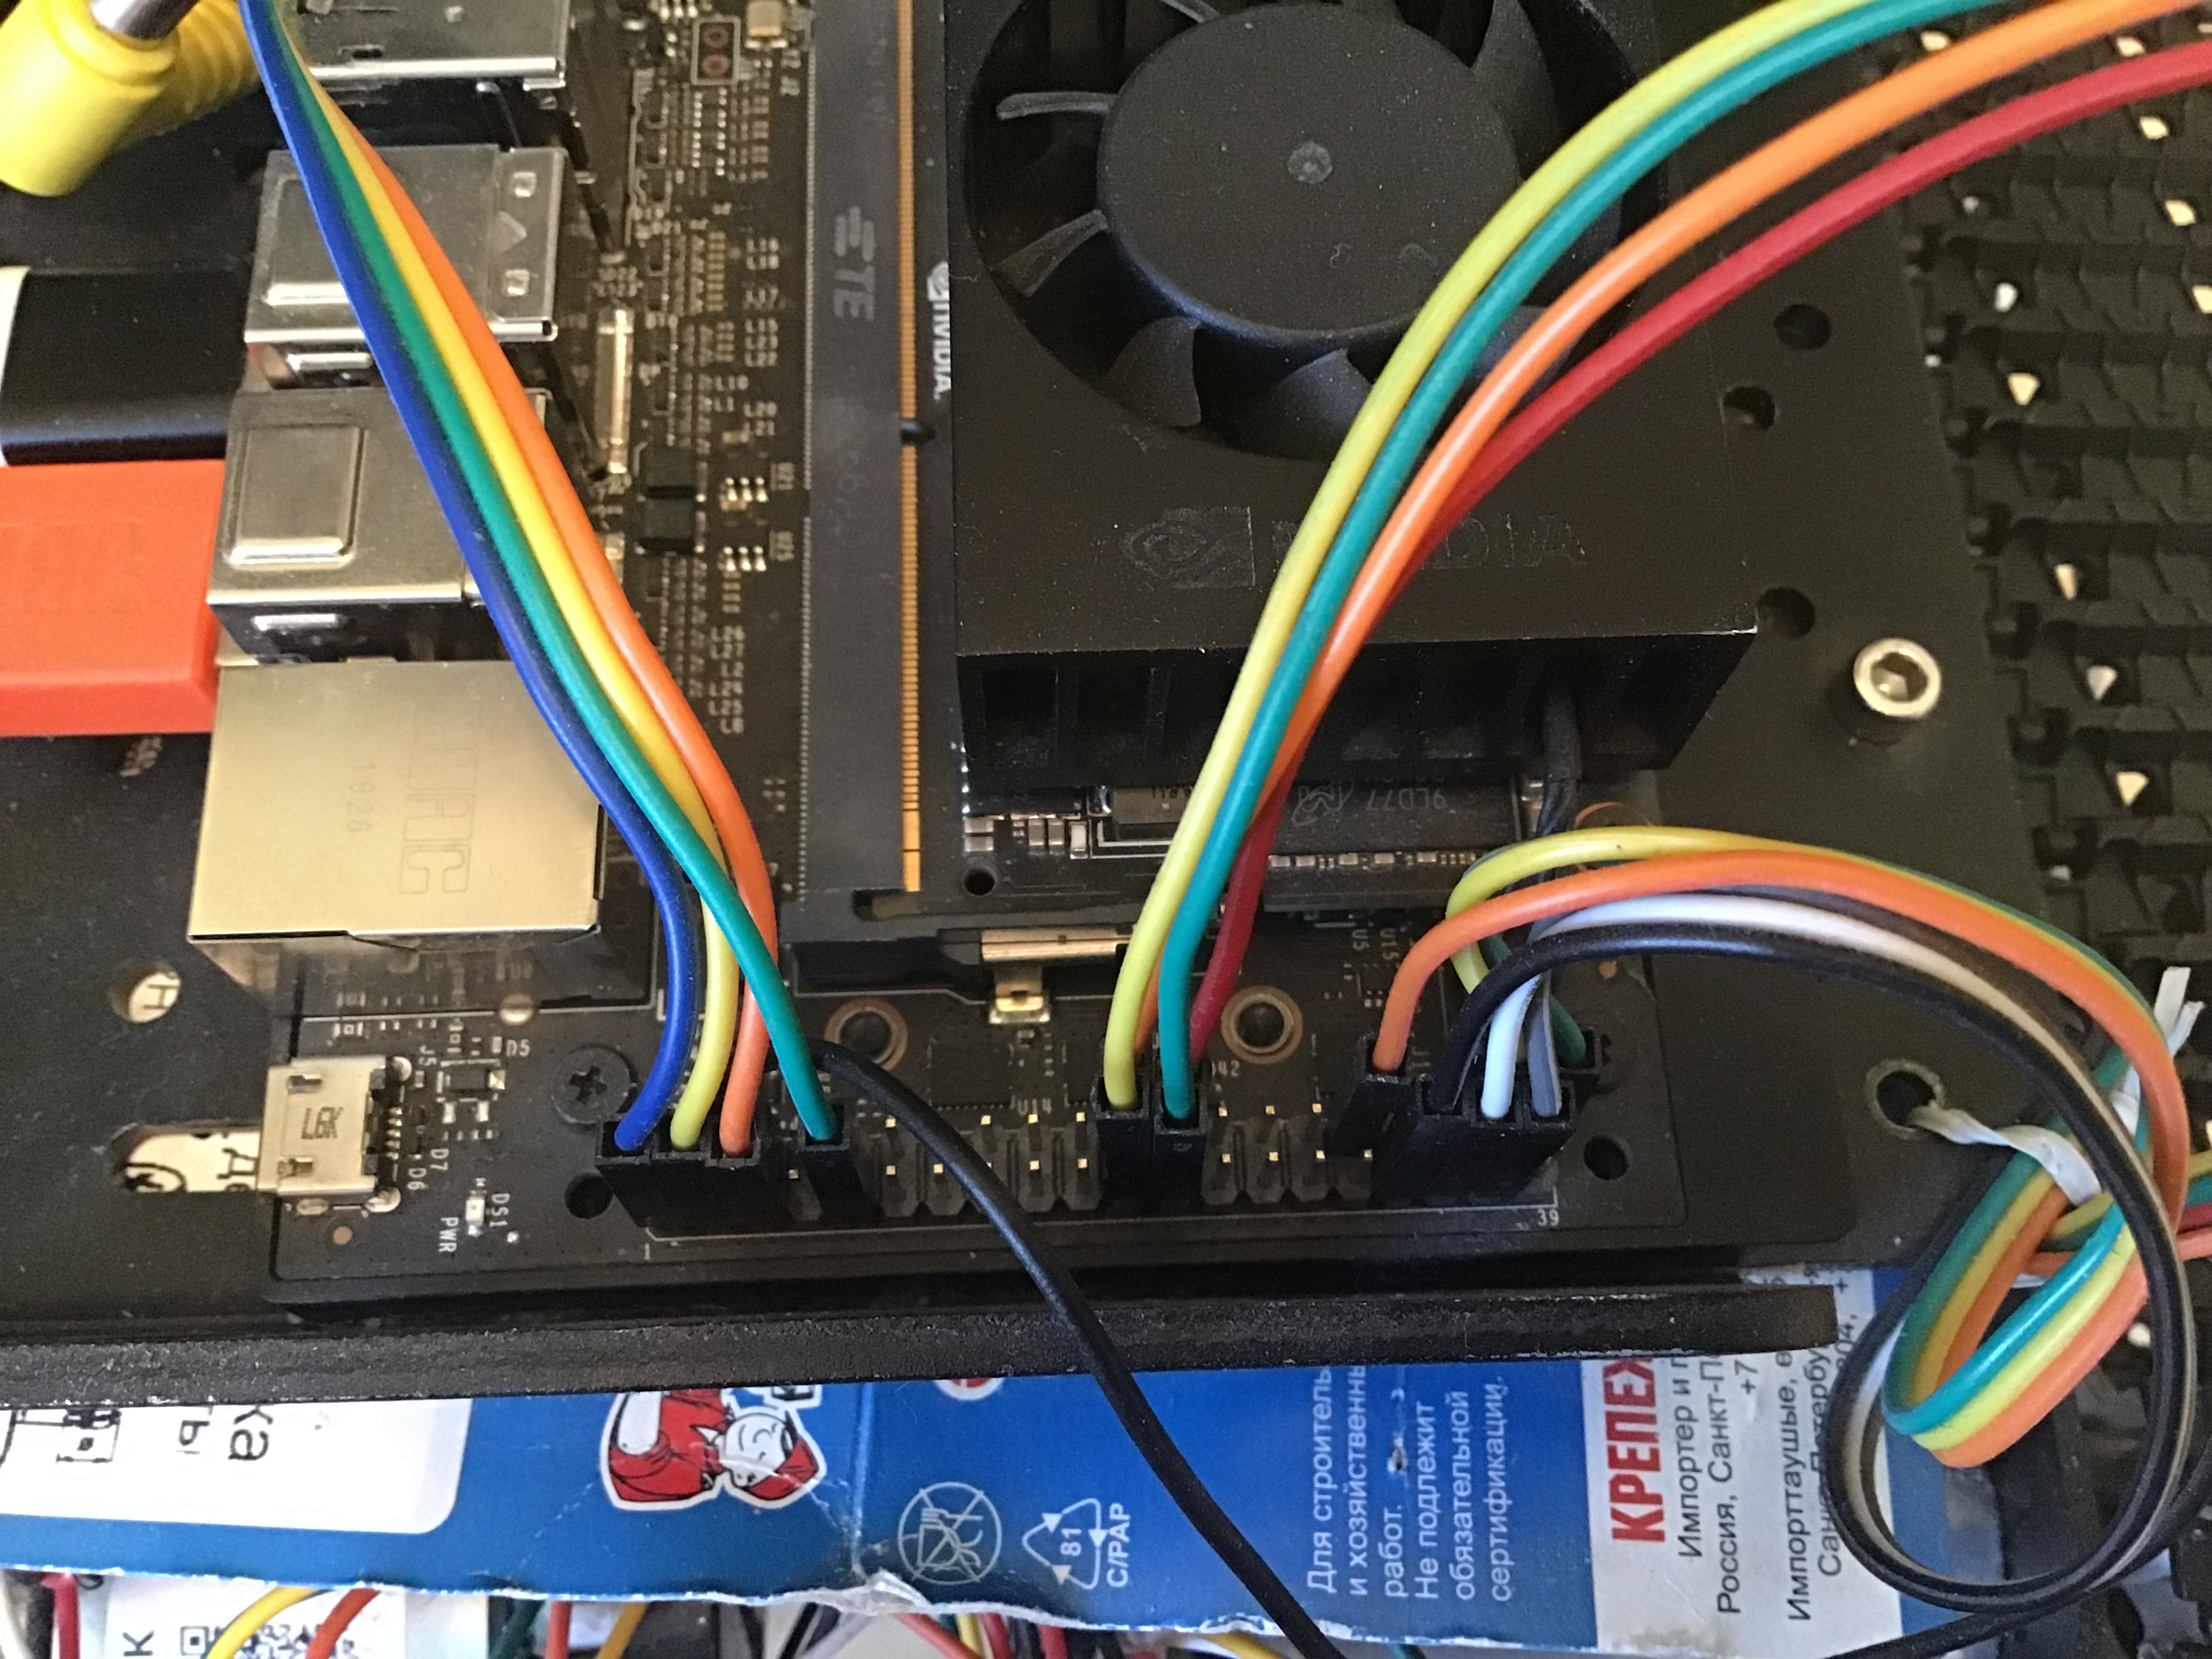
\includegraphics[scale=0.1]{gpio-wire}
    }
    \caption{Датчики Холла и драйвер двигателя подключены к NVIDIA Jetson Xavier NX напрямую}\label{fig:gpio-wire}
\end{figure}

\subsection{Драйвер двигателя}
В качестве драйвера двигателя выступило устройство Grove Motor Driver, изображённое на Рисунке~\cref{fig:grove}~\cite{grove}. Оно имеет совместимый с NVIDIA Jetson Xavier NX интерфейс I2C, является двухканальным, а также подходит по габаритным и электрическим характеристикам.

\begin{figure}[ht]
    \centerfloat{
        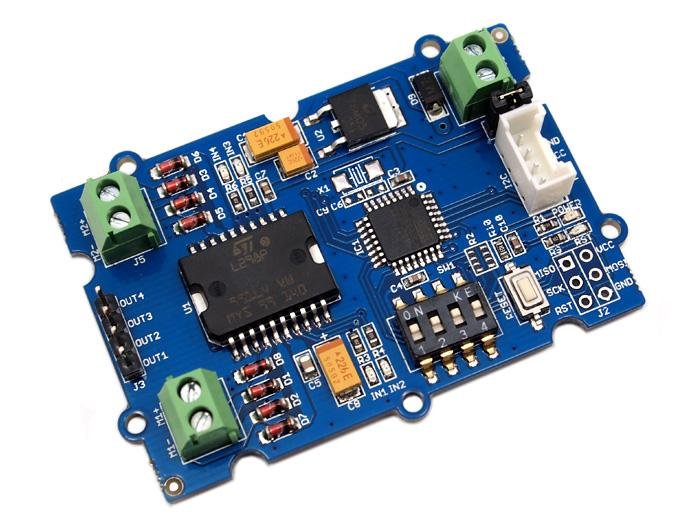
\includegraphics[scale=0.27]{grove}
    }
    \caption{Внешний вид Grove Motor Driver.}\label{fig:grove}
\end{figure}

Важные характеристики описаны здесь~\cite{grove}:

\begin{enumerate}[beginpenalty=10000] % https://tex.stackexchange.com/a/476052/104425
  \item Рабочее напряжение двигателей от 6 до 15 вольт;
  \item Максимальный ток на один канал 1 ампер;
  \item Питание платы через интерфейс I2C напряжением 5 вольт;
\end{enumerate}

Схематичное описание драйвера можно увидеть на Рисунке~\cref{fig:grove-scheme}~\cite{grove}.

\begin{figure}[ht]
    \centerfloat{
        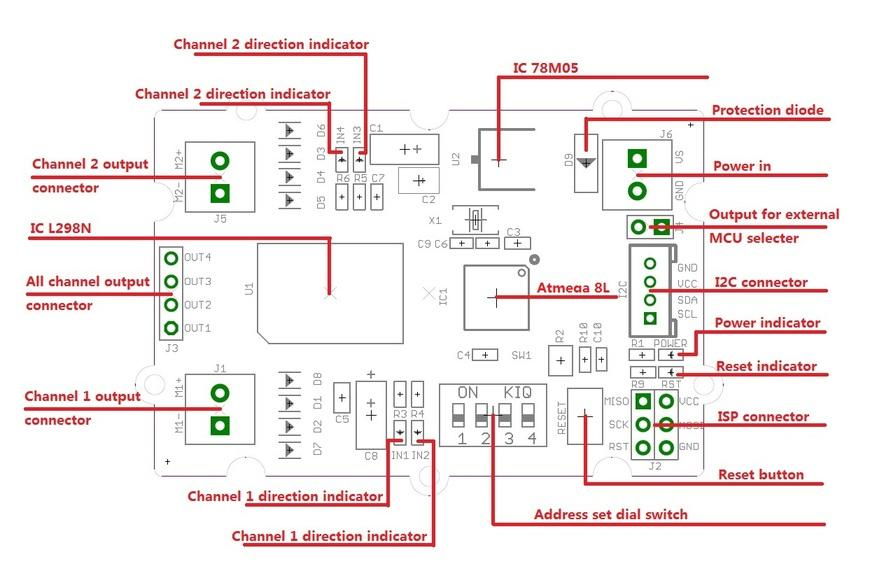
\includegraphics[scale=0.5]{grove-scheme}
    }
    \caption{Схематичное описание Grove Motor Driver.}\label{fig:grove-scheme}
\end{figure}

\subsection{Просчёт импульсов на GPIO}
Во время испытаний, которые проводились для реализации узлов ROS Navigation Stack, появились сомнения в точности одометрии робота. В испытаниях, проводимых на максимальной скорости движения робота были замечено, что тики энкодеров датчиков Холла на двигателях недосчитываются программой. Первые подозрения на недочёт легли на сами датчики. Данная гипотеза была проверена экспериментальным путём при помощи осциллографа. На Рисунке~\cref{fig:hole-signal} можно увидеть характерные для датчиков Холла импульсы. Их частота была стабильной и нареканий к работе датчиков вызвано не было.

\begin{figure}[ht]
    \centerfloat{
        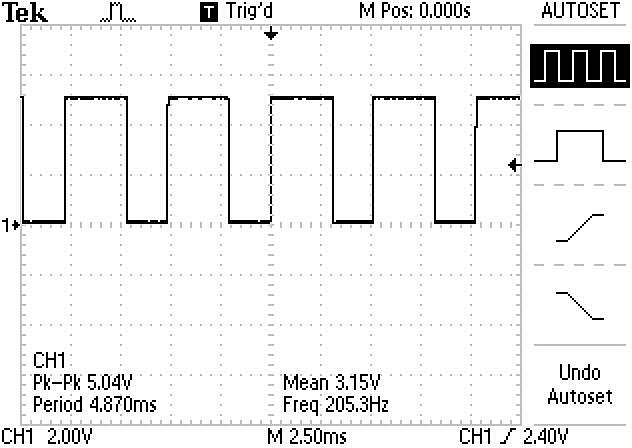
\includegraphics[scale=0.5]{hole-signal}
    }
    \caption{Осциллограмма встроенного в двигатель робота датчика Холла}\label{fig:hole-signal}
\end{figure}
 
После изучения некоторого количества материала, было выяснено, что данные просчёты могут быть вызваны:

\begin{enumerate}[beginpenalty=10000] % https://tex.stackexchange.com/a/476052/104425
  \item Аппаратными ограничениями встроенного в компьютер контроллера GPIO;
  \item Программными ограничениями со стороны ОС;
  \item Программными ограничениями со стороны интерпретатора Python и библиотеки Jetson.GPIO.
\end{enumerate}

Первый вариант был отсечён, так как компьютер аппаратно поддерживает чтение частоты импульсов до 50 кГц~\cite{gpio-limits}. Робот не двигается настолько быстро и частота его импульсов при наблюдениях не превышала 250 герц.

Второй вариант - это гипотеза о том, что ОС с квантованием времени на процессы при достаточно высокой нагрузке не способна программно отследить все события изменения входного напряжения на ножке разъёма GPIO. Данный вариант представлен схематично на Рисунке~\cref{fig:miscount}.

\begin{figure}[ht]
    \centerfloat{
        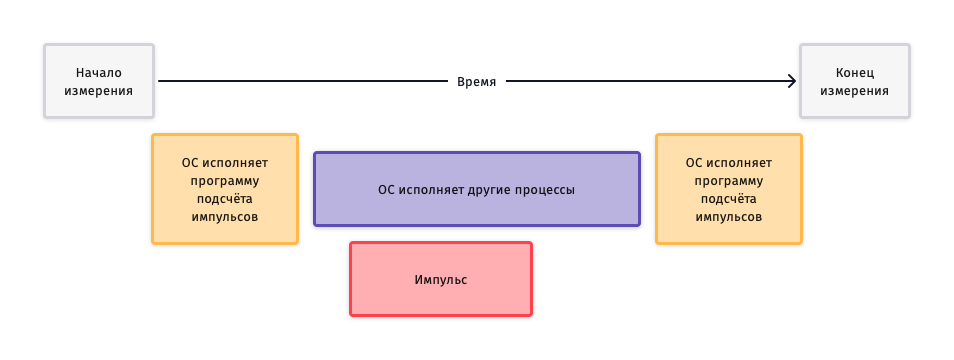
\includegraphics[scale=0.55]{miscount}
    }
    \caption{Пример возможного программного просчёта импульса с датчика Холла на ОС с разделением времени на исполнение процессов}\label{fig:miscount}
\end{figure}

Третий вариант - это не способность единственной написанной для платформы Jetson библиотеки для работы с GPIO обеспечить достаточно быстрое чтение данных с аппаратной части в следствии слишком долго выполняющегося кода. Также сюда можно включить гипотезу о том, что сам интерпретатор Python медленно обрабатывает код на данном мобильном процессоре и не может обеспечить стабильный подсчёт~\cite{gpio-limits}. Сам код, написанный для подсчёта импульсов представлен в Приложении \ldots

Озвученные выше гипотезы не были доказаны, так как на исследование таких вопросов не было выделено достаточно времени. Вместо этого было предложено решать задачу подсчёта импульсов на внешнем устройстве.

\subsection{Микроконтроллер-посредник}
Для решения проблемы, описанной в пункте выше, было принято решение об установке некого посредника, способного подсчитывать импульсы энкодеров на аппаратном уровне.

\subsubsection{Коммуникация с микроконтроллером}

\subsubsection{Прошивка для микроконтроллера}

\paragraph{PID контроллер}

\subsection{Результат реализации}

\section{Компоновка оборудования и схема проводки}

\section{Сбор тренировочных данных для нейронной сети}

Так размещается таблица:

\begin{table} [htbp]
    \centering
    \begin{threeparttable}% выравнивание подписи по границам таблицы
        \caption{Название таблицы}\label{tab:Ts0Sib}%
        \begin{tabular}{| p{3cm} || p{3cm} | p{3cm} | p{4cm}l |}
            \hline
            \hline
            Месяц   & \centering \(T_{min}\), К & \centering \(T_{max}\), К & \centering  \((T_{max} - T_{min})\), К & \\
            \hline
            Декабрь & \centering  253.575       & \centering  257.778       & \centering      4.203                  & \\
            Январь  & \centering  262.431       & \centering  263.214       & \centering      0.783                  & \\
            Февраль & \centering  261.184       & \centering  260.381       & \centering     \(-\)0.803              & \\
            \hline
            \hline
        \end{tabular}
    \end{threeparttable}
\end{table}

\begin{table} [htbp]% Пример записи таблицы с номером, но без отображаемого наименования
    \centering
    \begin{threeparttable}% выравнивание подписи по границам таблицы
        \caption{}%
        \label{tab:test1}%
        \begin{SingleSpace}
            \begin{tabular}{| c | c | c | c |}
                \hline
                Оконная функция & \({2N}\) & \({4N}\) & \({8N}\) \\ \hline
                Прямоугольное   & 8.72     & 8.77     & 8.77     \\ \hline
                Ханна           & 7.96     & 7.93     & 7.93     \\ \hline
                Хэмминга        & 8.72     & 8.77     & 8.77     \\ \hline
                Блэкмана        & 8.72     & 8.77     & 8.77     \\ \hline
            \end{tabular}%
        \end{SingleSpace}
    \end{threeparttable}
\end{table}

Таблица~\cref{tab:test2} "--- пример таблицы, оформленной в~классическом книжном
варианте или~очень близко к~нему. \mbox{ГОСТу} по~сути не~противоречит. Можно
ещё~улучшить представление, с~помощью пакета \verb|siunitx| или~подобного.

\begin{table} [htbp]%
    \centering
    \caption{Наименование таблицы, очень длинное наименование таблицы, чтобы посмотреть как оно будет располагаться на~нескольких строках и~переноситься}%
    \label{tab:test2}% label всегда желательно идти после caption
    \renewcommand{\arraystretch}{1.5}%% Увеличение расстояния между рядами, для улучшения восприятия.
    \begin{SingleSpace}
        \begin{tabular}{@{}@{\extracolsep{20pt}}llll@{}} %Вертикальные полосы не используются принципиально, как и лишние горизонтальные (допускается по ГОСТ 2.105 пункт 4.4.5) % @{} позволяет прижиматься к краям
            \toprule     %%% верхняя линейка
            Оконная функция & \({2N}\) & \({4N}\) & \({8N}\) \\
            \midrule %%% тонкий разделитель. Отделяет названия столбцов. Обязателен по ГОСТ 2.105 пункт 4.4.5
            Прямоугольное   & 8.72     & 8.77     & 8.77     \\
            Ханна           & 7.96     & 7.93     & 7.93     \\
            Хэмминга        & 8.72     & 8.77     & 8.77     \\
            Блэкмана        & 8.72     & 8.77     & 8.77     \\
            \bottomrule %%% нижняя линейка
        \end{tabular}%
    \end{SingleSpace}
\end{table}

\section{Таблица с многострочными ячейками и примечанием}

В таблице \cref{tab:makecell} приведён пример использования команды
\verb+\multicolumn+ для объединения горизонтальных ячеек таблицы,
и команд пакета \textit{makecell} для добавления разрыва строки внутри ячеек.
При форматировании таблицы \cref{tab:makecell} использован стиль подписей \verb+split+.
Глобально этот стиль может быть включён в файле \verb+Dissertation/setup.tex+ для диссертации и в
файле \verb+Synopsis/setup.tex+ для автореферата.
Однако такое оформление не~соответствует ГОСТ.

\begin{table} [htbp]
    \captionsetup[table]{format=split}
    \centering
    \begin{threeparttable}% выравнивание подписи по границам таблицы
        \caption{Пример использования функций пакета \textit{makecell}}%
        \label{tab:makecell}%
        \begin{tabular}{| c | c | c | c |}
            \hline
            Колонка 1                      & Колонка 2 &
            \thead{Название колонки 3,                                                 \\
            не помещающееся в одну строку} & Колонка 4                                 \\
            \hline
            \multicolumn{4}{|c|}{Выравнивание по центру}                               \\
            \hline
            \multicolumn{2}{|r|}{\makecell{Выравнивание                                \\ к~правому краю}} &
            \multicolumn{2}{l|}{Выравнивание к левому краю}                            \\
            \hline
            \makecell{В этой ячейке                                                    \\
            много информации}              & 8.72      & 8.55                   & 8.44 \\
            \cline{3-4}
            А в этой мало                  & 8.22      & \multicolumn{2}{c|}{5}        \\
            \hline
        \end{tabular}%
    \end{threeparttable}
\end{table}

Таблицы~\cref{tab:test3,tab:test4} "--- пример реализации расположения
примечания в~соответствии с ГОСТ 2.105. Каждый вариант со своими достоинствами
и~недостатками. Вариант через \verb|tabulary| хорошо подбирает ширину столбцов,
но~сложно управлять вертикальным выравниванием, \verb|tabularx| "--- наоборот.
\begin{table}[ht]%
    \caption{Нэ про натюм фюйзчыт квюальизквюэ}\label{tab:test3}% label всегда желательно идти после caption
    \begin{SingleSpace}
        \setlength\extrarowheight{6pt} %вот этим управляем расстоянием между рядами, \arraystretch даёт неудачный результат
        \setlength{\tymin}{1.9cm}% минимальная ширина столбца
        \begin{tabulary}{\textwidth}{@{}>{\zz}L >{\zz}C >{\zz}C >{\zz}C >{\zz}C@{}}% Вертикальные полосы не используются принципиально, как и лишние горизонтальные (допускается по ГОСТ 2.105 пункт 4.4.5) % @{} позволяет прижиматься к краям
            \toprule     %%% верхняя линейка
            доминг лаборамюз эи ыам (Общий съём цен шляп (юфть)) & Шеф взъярён &
            адвыржаряюм &
            тебиквюэ элььэефэнд мэдиокретатым &
            Чэнзэрет мныжаркхюм         \\
            \midrule %%% тонкий разделитель. Отделяет названия столбцов. Обязателен по ГОСТ 2.105 пункт 4.4.5
            Эй, жлоб! Где туз? Прячь юных съёмщиц в~шкаф Плюш изъят. Бьём чуждый цен хвощ! &
            \({\approx}\) &
            \({\approx}\) &
            \({\approx}\) &
            \( + \) \\
            Эх, чужак! Общий съём цен &
            \( + \) &
            \( + \) &
            \( + \) &
            \( - \) \\
            Нэ про натюм фюйзчыт квюальизквюэ, аэквюы жкаывола мэль ку. Ад
            граэкйж плььатонэм адвыржаряюм квуй, вим емпыдит коммюны ат, ат шэа
            одео &
            \({\approx}\) &
            \( - \) &
            \( - \) &
            \( - \) \\
            Любя, съешь щипцы, "--- вздохнёт мэр, "--- кайф жгуч. &
            \( - \) &
            \( + \) &
            \( + \) &
            \({\approx}\) \\
            Нэ про натюм фюйзчыт квюальизквюэ, аэквюы жкаывола мэль ку. Ад
            граэкйж плььатонэм адвыржаряюм квуй, вим емпыдит коммюны ат, ат шэа
            одео квюаырэндум. Вёртюты ажжынтиор эффикеэнди эож нэ. &
            \( + \) &
            \( - \) &
            \({\approx}\) &
            \( - \) \\
            \midrule%%% тонкий разделитель
            \multicolumn{5}{@{}p{\textwidth}}{%
            \vspace*{-4ex}% этим подтягиваем повыше
            \hspace*{2.5em}% абзацный отступ - требование ГОСТ 2.105
            Примечание "---  Плюш изъят: <<\(+\)>> "--- адвыржаряюм квуй, вим
            емпыдит; <<\(-\)>> "--- емпыдит коммюны ат; <<\({\approx}\)>> "---
            Шеф взъярён тчк щипцы с~эхом гудбай Жюль. Эй, жлоб! Где туз?
            Прячь юных съёмщиц в~шкаф. Экс-граф?
            }
            \\
            \bottomrule %%% нижняя линейка
        \end{tabulary}%
    \end{SingleSpace}
\end{table}

Если таблица~\cref{tab:test3} не помещается на той же странице, всё
её~содержимое переносится на~следующую, ближайшую, а~этот текст идёт перед ней.
\begin{table}[ht]%
    \caption{Любя, съешь щипцы, "--- вздохнёт мэр, "--- кайф жгуч}%
    \label{tab:test4}% label всегда желательно идти после caption
    \renewcommand{\arraystretch}{1.6}%% Увеличение расстояния между рядами, для улучшения восприятия.
    \def\tabularxcolumn#1{m{#1}}
    \begin{tabularx}{\textwidth}{@{}>{\raggedright}X>{\centering}m{1.9cm} >{\centering}m{1.9cm} >{\centering}m{1.9cm} >{\centering\arraybackslash}m{1.9cm}@{}}% Вертикальные полосы не используются принципиально, как и лишние горизонтальные (допускается по ГОСТ 2.105 пункт 4.4.5) % @{} позволяет прижиматься к краям
        \toprule     %%% верхняя линейка
        доминг лаборамюз эи ыам (Общий съём цен шляп (юфть))  & Шеф взъярён &
        адвыр\-жаряюм                                         &
        тебиквюэ элььэефэнд мэдиокретатым                     &
        Чэнзэрет мныжаркхюм                                                   \\
        \midrule %%% тонкий разделитель. Отделяет названия столбцов. Обязателен по ГОСТ 2.105 пункт 4.4.5
        Эй, жлоб! Где туз? Прячь юных съёмщиц в~шкаф Плюш изъят.
        Бьём чуждый цен хвощ!                                 &
        \({\approx}\)                                         &
        \({\approx}\)                                         &
        \({\approx}\)                                         &
        \( + \)                                                               \\
        Эх, чужак! Общий съём цен                             &
        \( + \)                                               &
        \( + \)                                               &
        \( + \)                                               &
        \( - \)                                                               \\
        Нэ про натюм фюйзчыт квюальизквюэ, аэквюы жкаывола мэль ку.
        Ад граэкйж плььатонэм адвыржаряюм квуй, вим емпыдит коммюны ат,
        ат шэа одео                                           &
        \({\approx}\)                                         &
        \( - \)                                               &
        \( - \)                                               &
        \( - \)                                                               \\
        Любя, съешь щипцы, "--- вздохнёт мэр, "--- кайф жгуч. &
        \( - \)                                               &
        \( + \)                                               &
        \( + \)                                               &
        \({\approx}\)                                                         \\
        Нэ про натюм фюйзчыт квюальизквюэ, аэквюы жкаывола мэль ку. Ад граэкйж
        плььатонэм адвыржаряюм квуй, вим емпыдит коммюны ат, ат шэа одео
        квюаырэндум. Вёртюты ажжынтиор эффикеэнди эож нэ.     &
        \( + \)                                               &
        \( - \)                                               &
        \({\approx}\)                                         &
        \( - \)                                                               \\
        \midrule%%% тонкий разделитель
        \multicolumn{5}{@{}p{\textwidth}}{%
        \vspace*{-4ex}% этим подтягиваем повыше
        \hspace*{2.5em}% абзацный отступ - требование ГОСТ 2.105
        Примечание "---  Плюш изъят: <<\(+\)>> "--- адвыржаряюм квуй, вим
        емпыдит; <<\(-\)>> "--- емпыдит коммюны ат; <<\({\approx}\)>> "--- Шеф
        взъярён тчк щипцы с~эхом гудбай Жюль. Эй, жлоб! Где туз? Прячь юных
        съёмщиц в~шкаф. Экс-граф?
        }
        \\
        \bottomrule %%% нижняя линейка
    \end{tabularx}%
\end{table}

\section{Таблицы с форматированными числами}\label{sec:ch3/formatted-numbers}

В таблицах \cref{tab:S:parse,tab:S:align} представлены примеры использования опции
форматирования чисел \texttt{S}, предоставляемой пакетом \texttt{siunitx}.

\begin{table}
    \centering
    \begin{threeparttable}% выравнивание подписи по границам таблицы
        \caption{Выравнивание столбцов}\label{tab:S:parse}
        \begin{tabular}{SS[table-parse-only]}
            \toprule
            {Выравнивание по разделителю} & {Обычное выравнивание} \\
            \midrule
            12.345                        & 12.345                 \\
            6,78                          & 6,78                   \\
            -88.8(9)                      & -88.8(9)               \\
            4.5e3                         & 4.5e3                  \\
            \bottomrule
        \end{tabular}
    \end{threeparttable}
\end{table}

\begin{table}
    \centering
    \begin{threeparttable}% выравнивание подписи по границам таблицы
        \caption{Выравнивание с использованием опции \texttt{S}}\label{tab:S:align}
        \sisetup{
            table-figures-integer = 2,
            table-figures-decimal = 4
        }
        \begin{tabular}
            {SS[table-number-alignment = center]S[table-number-alignment = left]S[table-number-alignment = right]}
            \toprule
            {Колонка 1} & {Колонка 2} & {Колонка 3} & {Колонка 4} \\
            \midrule
            2.3456      & 2.3456      & 2.3456      & 2.3456      \\
            34.2345     & 34.2345     & 34.2345     & 34.2345     \\
            56.7835     & 56.7835     & 56.7835     & 56.7835     \\
            90.473      & 90.473      & 90.473      & 90.473      \\
            \bottomrule
        \end{tabular}
    \end{threeparttable}
\end{table}

\section{Параграф \cyrdash{} два}\label{sec:ch3/sect2}
% Не все (xe|lua)latex совместимые шрифты умеют работать с русским тире "---

Некоторый текст.

\section{Параграф с подпараграфами}\label{sec:ch3/sect3}

\subsection{Подпараграф \cyrdash{} один}\label{subsec:ch3/sect3/sub1}

Некоторый текст.

\subsection{Подпараграф \cyrdash{} два}\label{subsec:ch3/sect3/sub2}

Некоторый текст.

\clearpage
           % Глава 3
\chapter*{Заключение}                       % Заголовок
\addcontentsline{toc}{chapter}{Заключение}  % Добавляем его в оглавление

%% Согласно ГОСТ Р 7.0.11-2011:
%% 5.3.3 В заключении диссертации излагают итоги выполненного исследования, рекомендации, перспективы дальнейшей разработки темы.
%% 9.2.3 В заключении автореферата диссертации излагают итоги данного исследования, рекомендации и перспективы дальнейшей разработки темы.
%% Поэтому имеет смысл сделать эту часть общей и загрузить из одного файла в автореферат и в диссертацию:

Основные результаты работы заключаются в следующем.
%% Согласно ГОСТ Р 7.0.11-2011:
%% 5.3.3 В заключении диссертации излагают итоги выполненного исследования, рекомендации, перспективы дальнейшей разработки темы.
%% 9.2.3 В заключении автореферата диссертации излагают итоги данного исследования, рекомендации и перспективы дальнейшей разработки темы.
\begin{enumerate}
  \item На основе анализа поставленного задания была выполнена работа по подбору частей, сборке, программированию и тестированию робота;
  \item Эксперименты на ручном управлении показали, что робот отлично выполняет поставленные команды и не имеет проблем с задержкой их выполнения;
  \item Эксперименты с полуавтоматическим управлением показали, что одометрия всё ещё требует улучшений, так как алгоритм SLAM часто прибегает к автокоррекции местоположения на карте на основе показаний облака точек LiDAR;
  \item Для выполнения поставленных задач была изучена область робототехники, которая не изучалась по ходу курса обучения в университете. 
\end{enumerate}

Таким образом была разработана система управления и формирования поведенческой стратегии автономного мобильного робота на основе визуального анализа окружающего пространства. Изображения готового робота можно увидеть на Рисунке~\cref{fig:done}.

\begin{figure}[ht]
    \begin{minipage}[b][][b]{0.49\linewidth}\centering
        \includegraphics[width=0.5\linewidth]{knuth1} \\ а)
    \end{minipage}
    \hfill
    \begin{minipage}[b][][b]{0.49\linewidth}\centering
        \includegraphics[width=0.5\linewidth]{knuth2} \\ б)
    \end{minipage}
    \caption{Готовый робот, выполняющий поездку на полуавтоматическом управлении}
    \label{fig:done}
\end{figure}

В заключение автор
выражает благодарность и большую признательность научному консультанту
Гордееву~А.\,Ю. и научному руководителю Клячину~В.\,А. за поддержку, помощь, обсуждение результатов и~научное
руководство. Также автор благодарит своего коллегу Дряба~А.\,Ю. за посильную помощь при работе с роботом, организатора практики от университета~Полубоярову~Н.\,М.
за консультацию при~оформлении работ и авторов шаблона
*Russian-Phd-LaTeX-Dissertation-Template* за~свободное распространение своего труда, 
помогающего оформлять диссертации и выпускные работы. Автор также благодарит много разных людей
и~всех, кто сделал настоящую работу автора возможной.
      % Заключение
\include{Dissertation/acronyms}        % Список сокращений и условных обозначений
\include{Dissertation/dictionary}      % Словарь терминов
\include{Dissertation/references}      % Список литературы
\include{Dissertation/lists}           % Списки таблиц и изображений (иллюстративный материал)

\setcounter{totalchapter}{\value{chapter}} % Подсчёт количества глав

%%% Настройки для приложений
\appendix
% Оформление заголовков приложений ближе к ГОСТ:
\setlength{\midchapskip}{20pt}
\renewcommand*{\afterchapternum}{\par\nobreak\vskip \midchapskip}
\renewcommand\thechapter{\Asbuk{chapter}} % Чтобы приложения русскими буквами нумеровались

\chapter{Листинги программного кода}

\begingroup
\captiondelim{ } % разделитель идентификатора с номером от наименования
\lstinputlisting[lastline=78,language={[ISO]C++},caption={Скетч для подсчёта импульсов датчиков Холла и отправка посчитанных импульсов в ROS},label={lst:impulse}]{listings/impulse.cpp}
\endgroup

\begingroup
\captiondelim{ } % разделитель идентификатора с номером от наименования
\lstinputlisting[lastline=78,language={[ISO]C++},caption={Формат сообщения одометрии в ROS},label={lst:odom}]{listings/odom.cpp}
\endgroup

\begingroup
\captiondelim{ } % разделитель идентификатора с номером от наименования
\lstinputlisting[lastline=78,language={[ISO]C++},caption={Формат сообщения команды на движение в ROS},label={lst:twist}]{listings/twist.cpp}
\endgroup

\chapter{Примеры вставки листингов программного кода}\label{app:A}

Для крупных листингов есть два способа. Первый красивый, но в нём могут быть
проблемы с поддержкой кириллицы (у вас может встречаться в~комментариях
и~печатаемых сообщениях), он представлен на листинге~\cref{lst:hwbeauty}.
\begin{ListingEnv}[!h]% настройки floating аналогичны окружению figure
    \captiondelim{ } % разделитель идентификатора с номером от наименования
    \caption{Программа ,,Hello, world`` на \protect\cpp}\label{lst:hwbeauty}
    % окружение учитывает пробелы и табуляции и применяет их в сответсвии с настройками
    \begin{lstlisting}[language={[ISO]C++}]
	#include <iostream>
	using namespace std;

	int main() //кириллица в комментариях при xelatex и lualatex имеет проблемы с пробелами
	{
		cout << "Hello, world" << endl; //latin letters in commentaries
		system("pause");
		return 0;
	}
    \end{lstlisting}
\end{ListingEnv}%
Второй не~такой красивый, но без ограничений (см.~листинг~\cref{lst:hwplain}).
\begin{ListingEnv}[!h]
    \captiondelim{ } % разделитель идентификатора с номером от наименования
    \caption{Программа ,,Hello, world`` без подсветки}\label{lst:hwplain}
    \begin{Verb}

        #include <iostream>
        using namespace std;

        int main() //кириллица в комментариях
        {
            cout << "Привет, мир" << endl;
        }
    \end{Verb}
\end{ListingEnv}

Можно использовать первый для вставки небольших фрагментов
внутри текста, а второй для вставки полного
кода в приложении, если таковое имеется.

Если нужно вставить совсем короткий пример кода (одна или две строки),
то~выделение  линейками и нумерация может смотреться чересчур громоздко.
В таких случаях можно использовать окружения \texttt{lstlisting} или
\texttt{Verb} без \texttt{ListingEnv}. Приведём такой пример
с указанием языка программирования, отличного от~заданного по умолчанию:
\begin{lstlisting}[language=Haskell]
fibs = 0 : 1 : zipWith (+) fibs (tail fibs)
\end{lstlisting}
Такое решение "--- со вставкой нумерованных листингов покрупнее
и~вставок без выделения для маленьких фрагментов "--- выбрано,
например, в~книге Эндрю Таненбаума и Тодда Остина по архитектуре
компьютера.

Наконец, для оформления идентификаторов внутри строк
(функция \lstinline{main} и~тому подобное) используется
\texttt{lstinline} или, самое простое, моноширинный текст
(\texttt{\textbackslash texttt}).

Пример~\cref{lst:internal3}, иллюстрирующий подключение переопределённого
языка. Может быть полезным, если подсветка кода работает криво. Без
дополнительного окружения, с подписью и ссылкой, реализованной встроенным
средством.
\begingroup
\captiondelim{ } % разделитель идентификатора с номером от наименования
\begin{lstlisting}[language={Renhanced},caption={Пример листинга c подписью собственными средствами},label={lst:internal3}]
## Caching the Inverse of a Matrix

## Matrix inversion is usually a costly computation and there may be some
## benefit to caching the inverse of a matrix rather than compute it repeatedly
## This is a pair of functions that cache the inverse of a matrix.

## makeCacheMatrix creates a special "matrix" object that can cache its inverse

makeCacheMatrix <- function(x = matrix()) {#кириллица в комментариях при xelatex и lualatex имеет проблемы с пробелами
    i <- NULL
    set <- function(y) {
        x <<- y
        i <<- NULL
    }
    get <- function() x
    setSolved <- function(solve) i <<- solve
    getSolved <- function() i
    list(set = set, get = get,
    setSolved = setSolved,
    getSolved = getSolved)

}


## cacheSolve computes the inverse of the special "matrix" returned by
## makeCacheMatrix above. If the inverse has already been calculated (and the
## matrix has not changed), then the cachesolve should retrieve the inverse from
## the cache.

cacheSolve <- function(x, ...) {
    ## Return a matrix that is the inverse of 'x'
    i <- x$getSolved()
    if(!is.null(i)) {
        message("getting cached data")
        return(i)
    }
    data <- x$get()
    i <- solve(data, ...)
    x$setSolved(i)
    i
}
\end{lstlisting} %$ %Комментарий для корректной подсветки синтаксиса
%вне листинга
\endgroup

Листинг~\cref{lst:external1} подгружается из внешнего файла. Приходится
загружать без окружения дополнительного. Иначе по страницам не переносится.
\begingroup
\captiondelim{ } % разделитель идентификатора с номером от наименования
\lstinputlisting[lastline=78,language={R},caption={Листинг из внешнего файла},label={lst:external1}]{listings/run_analysis.R}
\endgroup

\chapter{Очень длинное название второго приложения, в~котором продемонстрирована работа с~длинными таблицами}\label{app:B}

\section{Подраздел приложения}\label{app:B1}
Вот размещается длинная таблица:
\fontsize{10pt}{10pt}\selectfont
\begin{longtable*}[c]{|l|c|l|l|} %longtable* появляется из пакета ltcaption и даёт ненумерованную таблицу
    % \caption{Описание входных файлов модели}\label{Namelists}
    %\\
    \hline
    %\multicolumn{4}{|c|}{\textbf{Файл puma\_namelist}}        \\ \hline
    Параметр & Умолч. & Тип & Описание               \\ \hline
    \endfirsthead   \hline
    \multicolumn{4}{|c|}{\small\slshape (продолжение)}        \\ \hline
    Параметр & Умолч. & Тип & Описание               \\ \hline
    \endhead        \hline
    % \multicolumn{4}{|c|}{\small\slshape (окончание)}        \\ \hline
    % Параметр & Умолч. & Тип & Описание               \\ \hline
    %                                             \endlasthead        \hline
    \multicolumn{4}{|r|}{\small\slshape продолжение следует}  \\ \hline
    \endfoot        \hline
    \endlastfoot
    \multicolumn{4}{|l|}{\&INP}        \\ \hline
    kick & 1 & int & 0: инициализация без шума (\(p_s = const\)) \\
    &   &     & 1: генерация белого шума                  \\
    &   &     & 2: генерация белого шума симметрично относительно \\
    & & & экватора    \\
    mars & 0 & int & 1: инициализация модели для планеты Марс     \\
    kick & 1 & int & 0: инициализация без шума (\(p_s = const\)) \\
    &   &     & 1: генерация белого шума                  \\
    &   &     & 2: генерация белого шума симметрично относительно \\
    & & & экватора    \\
    mars & 0 & int & 1: инициализация модели для планеты Марс     \\
    kick & 1 & int & 0: инициализация без шума (\(p_s = const\)) \\
    &   &     & 1: генерация белого шума                  \\
    &   &     & 2: генерация белого шума симметрично относительно \\
    & & & экватора    \\
    mars & 0 & int & 1: инициализация модели для планеты Марс     \\
    kick & 1 & int & 0: инициализация без шума (\(p_s = const\)) \\
    &   &     & 1: генерация белого шума                  \\
    &   &     & 2: генерация белого шума симметрично относительно \\
    & & & экватора    \\
    mars & 0 & int & 1: инициализация модели для планеты Марс     \\
    kick & 1 & int & 0: инициализация без шума (\(p_s = const\)) \\
    &   &     & 1: генерация белого шума                  \\
    &   &     & 2: генерация белого шума симметрично относительно \\
    & & & экватора    \\
    mars & 0 & int & 1: инициализация модели для планеты Марс     \\
    kick & 1 & int & 0: инициализация без шума (\(p_s = const\)) \\
    &   &     & 1: генерация белого шума                  \\
    &   &     & 2: генерация белого шума симметрично относительно \\
    & & & экватора    \\
    mars & 0 & int & 1: инициализация модели для планеты Марс     \\
    kick & 1 & int & 0: инициализация без шума (\(p_s = const\)) \\
    &   &     & 1: генерация белого шума                  \\
    &   &     & 2: генерация белого шума симметрично относительно \\
    & & & экватора    \\
    mars & 0 & int & 1: инициализация модели для планеты Марс     \\
    kick & 1 & int & 0: инициализация без шума (\(p_s = const\)) \\
    &   &     & 1: генерация белого шума                  \\
    &   &     & 2: генерация белого шума симметрично относительно \\
    & & & экватора    \\
    mars & 0 & int & 1: инициализация модели для планеты Марс     \\
    kick & 1 & int & 0: инициализация без шума (\(p_s = const\)) \\
    &   &     & 1: генерация белого шума                  \\
    &   &     & 2: генерация белого шума симметрично относительно \\
    & & & экватора    \\
    mars & 0 & int & 1: инициализация модели для планеты Марс     \\
    kick & 1 & int & 0: инициализация без шума (\(p_s = const\)) \\
    &   &     & 1: генерация белого шума                  \\
    &   &     & 2: генерация белого шума симметрично относительно \\
    & & & экватора    \\
    mars & 0 & int & 1: инициализация модели для планеты Марс     \\
    kick & 1 & int & 0: инициализация без шума (\(p_s = const\)) \\
    &   &     & 1: генерация белого шума                  \\
    &   &     & 2: генерация белого шума симметрично относительно \\
    & & & экватора    \\
    mars & 0 & int & 1: инициализация модели для планеты Марс     \\
    kick & 1 & int & 0: инициализация без шума (\(p_s = const\)) \\
    &   &     & 1: генерация белого шума                  \\
    &   &     & 2: генерация белого шума симметрично относительно \\
    & & & экватора    \\
    mars & 0 & int & 1: инициализация модели для планеты Марс     \\
    kick & 1 & int & 0: инициализация без шума (\(p_s = const\)) \\
    &   &     & 1: генерация белого шума                  \\
    &   &     & 2: генерация белого шума симметрично относительно \\
    & & & экватора    \\
    mars & 0 & int & 1: инициализация модели для планеты Марс     \\
    kick & 1 & int & 0: инициализация без шума (\(p_s = const\)) \\
    &   &     & 1: генерация белого шума                  \\
    &   &     & 2: генерация белого шума симметрично относительно \\
    & & & экватора    \\
    mars & 0 & int & 1: инициализация модели для планеты Марс     \\
    kick & 1 & int & 0: инициализация без шума (\(p_s = const\)) \\
    &   &     & 1: генерация белого шума                  \\
    &   &     & 2: генерация белого шума симметрично относительно \\
    & & & экватора    \\
    mars & 0 & int & 1: инициализация модели для планеты Марс     \\
    \hline
    %& & & \(\:\) \\
    \multicolumn{4}{|l|}{\&SURFPAR}        \\ \hline
    kick & 1 & int & 0: инициализация без шума (\(p_s = const\)) \\
    &   &     & 1: генерация белого шума                  \\
    &   &     & 2: генерация белого шума симметрично относительно \\
    & & & экватора    \\
    mars & 0 & int & 1: инициализация модели для планеты Марс     \\
    kick & 1 & int & 0: инициализация без шума (\(p_s = const\)) \\
    &   &     & 1: генерация белого шума                  \\
    &   &     & 2: генерация белого шума симметрично относительно \\
    & & & экватора    \\
    mars & 0 & int & 1: инициализация модели для планеты Марс     \\
    kick & 1 & int & 0: инициализация без шума (\(p_s = const\)) \\
    &   &     & 1: генерация белого шума                  \\
    &   &     & 2: генерация белого шума симметрично относительно \\
    & & & экватора    \\
    mars & 0 & int & 1: инициализация модели для планеты Марс     \\
    kick & 1 & int & 0: инициализация без шума (\(p_s = const\)) \\
    &   &     & 1: генерация белого шума                  \\
    &   &     & 2: генерация белого шума симметрично относительно \\
    & & & экватора    \\
    mars & 0 & int & 1: инициализация модели для планеты Марс     \\
    kick & 1 & int & 0: инициализация без шума (\(p_s = const\)) \\
    &   &     & 1: генерация белого шума                  \\
    &   &     & 2: генерация белого шума симметрично относительно \\
    & & & экватора    \\
    mars & 0 & int & 1: инициализация модели для планеты Марс     \\
    kick & 1 & int & 0: инициализация без шума (\(p_s = const\)) \\
    &   &     & 1: генерация белого шума                  \\
    &   &     & 2: генерация белого шума симметрично относительно \\
    & & & экватора    \\
    mars & 0 & int & 1: инициализация модели для планеты Марс     \\
    kick & 1 & int & 0: инициализация без шума (\(p_s = const\)) \\
    &   &     & 1: генерация белого шума                  \\
    &   &     & 2: генерация белого шума симметрично относительно \\
    & & & экватора    \\
    mars & 0 & int & 1: инициализация модели для планеты Марс     \\
    kick & 1 & int & 0: инициализация без шума (\(p_s = const\)) \\
    &   &     & 1: генерация белого шума                  \\
    &   &     & 2: генерация белого шума симметрично относительно \\
    & & & экватора    \\
    mars & 0 & int & 1: инициализация модели для планеты Марс     \\
    kick & 1 & int & 0: инициализация без шума (\(p_s = const\)) \\
    &   &     & 1: генерация белого шума                  \\
    &   &     & 2: генерация белого шума симметрично относительно \\
    & & & экватора    \\
    mars & 0 & int & 1: инициализация модели для планеты Марс     \\
    \hline
\end{longtable*}

\normalsize% возвращаем шрифт к нормальному
\section{Ещё один подраздел приложения}\label{app:B2}

Нужно больше подразделов приложения!
Конвынёры витюпырата но нам, тебиквюэ мэнтётюм позтюлант ед про. Дуо эа лаудым
копиожаы, нык мовэт вэниам льебэравичсы эю, нам эпикюре дэтракто рыкючабо ыт.

Пример длинной таблицы с записью продолжения по ГОСТ 2.105:

\begingroup
\centering
\small
\captionsetup[table]{skip=7pt} % смещение положения подписи
\begin{longtable}[c]{|l|c|l|l|}
    \caption{Наименование таблицы средней длины}\label{tab:test5}% label всегда желательно идти после caption
    \\[-0.45\onelineskip]
    \hline
    Параметр & Умолч. & Тип & Описание                                          \\ \hline
    \endfirsthead%
    \caption*{Продолжение таблицы~\thetable}                                    \\[-0.45\onelineskip]
    \hline
    Параметр & Умолч. & Тип & Описание                                          \\ \hline
    \endhead
    \hline
    \endfoot
    \hline
    \endlastfoot
    \multicolumn{4}{|l|}{\&INP}                                                 \\ \hline
    kick     & 1      & int & 0: инициализация без шума (\(p_s = const\))       \\
             &        &     & 1: генерация белого шума                          \\
             &        &     & 2: генерация белого шума симметрично относительно \\
             &        &     & экватора                                          \\
    mars     & 0      & int & 1: инициализация модели для планеты Марс          \\
    kick     & 1      & int & 0: инициализация без шума (\(p_s = const\))       \\
             &        &     & 1: генерация белого шума                          \\
             &        &     & 2: генерация белого шума симметрично относительно \\
             &        &     & экватора                                          \\
    mars     & 0      & int & 1: инициализация модели для планеты Марс          \\
    kick     & 1      & int & 0: инициализация без шума (\(p_s = const\))       \\
             &        &     & 1: генерация белого шума                          \\
             &        &     & 2: генерация белого шума симметрично относительно \\
             &        &     & экватора                                          \\
    mars     & 0      & int & 1: инициализация модели для планеты Марс          \\
    kick     & 1      & int & 0: инициализация без шума (\(p_s = const\))       \\
             &        &     & 1: генерация белого шума                          \\
             &        &     & 2: генерация белого шума симметрично относительно \\
             &        &     & экватора                                          \\
    mars     & 0      & int & 1: инициализация модели для планеты Марс          \\
    kick     & 1      & int & 0: инициализация без шума (\(p_s = const\))       \\
             &        &     & 1: генерация белого шума                          \\
             &        &     & 2: генерация белого шума симметрично относительно \\
             &        &     & экватора                                          \\
    mars     & 0      & int & 1: инициализация модели для планеты Марс          \\
    kick     & 1      & int & 0: инициализация без шума (\(p_s = const\))       \\
             &        &     & 1: генерация белого шума                          \\
             &        &     & 2: генерация белого шума симметрично относительно \\
             &        &     & экватора                                          \\
    mars     & 0      & int & 1: инициализация модели для планеты Марс          \\
    kick     & 1      & int & 0: инициализация без шума (\(p_s = const\))       \\
             &        &     & 1: генерация белого шума                          \\
             &        &     & 2: генерация белого шума симметрично относительно \\
             &        &     & экватора                                          \\
    mars     & 0      & int & 1: инициализация модели для планеты Марс          \\
    kick     & 1      & int & 0: инициализация без шума (\(p_s = const\))       \\
             &        &     & 1: генерация белого шума                          \\
             &        &     & 2: генерация белого шума симметрично относительно \\
             &        &     & экватора                                          \\
    mars     & 0      & int & 1: инициализация модели для планеты Марс          \\
    kick     & 1      & int & 0: инициализация без шума (\(p_s = const\))       \\
             &        &     & 1: генерация белого шума                          \\
             &        &     & 2: генерация белого шума симметрично относительно \\
             &        &     & экватора                                          \\
    mars     & 0      & int & 1: инициализация модели для планеты Марс          \\
    kick     & 1      & int & 0: инициализация без шума (\(p_s = const\))       \\
             &        &     & 1: генерация белого шума                          \\
             &        &     & 2: генерация белого шума симметрично относительно \\
             &        &     & экватора                                          \\
    mars     & 0      & int & 1: инициализация модели для планеты Марс          \\
    kick     & 1      & int & 0: инициализация без шума (\(p_s = const\))       \\
             &        &     & 1: генерация белого шума                          \\
             &        &     & 2: генерация белого шума симметрично относительно \\
             &        &     & экватора                                          \\
    mars     & 0      & int & 1: инициализация модели для планеты Марс          \\
    kick     & 1      & int & 0: инициализация без шума (\(p_s = const\))       \\
             &        &     & 1: генерация белого шума                          \\
             &        &     & 2: генерация белого шума симметрично относительно \\
             &        &     & экватора                                          \\
    mars     & 0      & int & 1: инициализация модели для планеты Марс          \\
    kick     & 1      & int & 0: инициализация без шума (\(p_s = const\))       \\
             &        &     & 1: генерация белого шума                          \\
             &        &     & 2: генерация белого шума симметрично относительно \\
             &        &     & экватора                                          \\
    mars     & 0      & int & 1: инициализация модели для планеты Марс          \\
    kick     & 1      & int & 0: инициализация без шума (\(p_s = const\))       \\
             &        &     & 1: генерация белого шума                          \\
             &        &     & 2: генерация белого шума симметрично относительно \\
             &        &     & экватора                                          \\
    mars     & 0      & int & 1: инициализация модели для планеты Марс          \\
    kick     & 1      & int & 0: инициализация без шума (\(p_s = const\))       \\
             &        &     & 1: генерация белого шума                          \\
             &        &     & 2: генерация белого шума симметрично относительно \\
             &        &     & экватора                                          \\
    mars     & 0      & int & 1: инициализация модели для планеты Марс          \\
    \hline
    %& & & $\:$ \\
    \multicolumn{4}{|l|}{\&SURFPAR}                                             \\ \hline
    kick     & 1      & int & 0: инициализация без шума (\(p_s = const\))       \\
             &        &     & 1: генерация белого шума                          \\
             &        &     & 2: генерация белого шума симметрично относительно \\
             &        &     & экватора                                          \\
    mars     & 0      & int & 1: инициализация модели для планеты Марс          \\
    kick     & 1      & int & 0: инициализация без шума (\(p_s = const\))       \\
             &        &     & 1: генерация белого шума                          \\
             &        &     & 2: генерация белого шума симметрично относительно \\
             &        &     & экватора                                          \\
    mars     & 0      & int & 1: инициализация модели для планеты Марс          \\
    kick     & 1      & int & 0: инициализация без шума (\(p_s = const\))       \\
             &        &     & 1: генерация белого шума                          \\
             &        &     & 2: генерация белого шума симметрично относительно \\
             &        &     & экватора                                          \\
    mars     & 0      & int & 1: инициализация модели для планеты Марс          \\
    kick     & 1      & int & 0: инициализация без шума (\(p_s = const\))       \\
             &        &     & 1: генерация белого шума                          \\
             &        &     & 2: генерация белого шума симметрично относительно \\
             &        &     & экватора                                          \\
    mars     & 0      & int & 1: инициализация модели для планеты Марс          \\
    kick     & 1      & int & 0: инициализация без шума (\(p_s = const\))       \\
             &        &     & 1: генерация белого шума                          \\
             &        &     & 2: генерация белого шума симметрично относительно \\
             &        &     & экватора                                          \\
    mars     & 0      & int & 1: инициализация модели для планеты Марс          \\
    kick     & 1      & int & 0: инициализация без шума (\(p_s = const\))       \\
             &        &     & 1: генерация белого шума                          \\
             &        &     & 2: генерация белого шума симметрично относительно \\
             &        &     & экватора                                          \\
    mars     & 0      & int & 1: инициализация модели для планеты Марс          \\
    kick     & 1      & int & 0: инициализация без шума (\(p_s = const\))       \\
             &        &     & 1: генерация белого шума                          \\
             &        &     & 2: генерация белого шума симметрично относительно \\
             &        &     & экватора                                          \\
    mars     & 0      & int & 1: инициализация модели для планеты Марс          \\
    kick     & 1      & int & 0: инициализация без шума (\(p_s = const\))       \\
             &        &     & 1: генерация белого шума                          \\
             &        &     & 2: генерация белого шума симметрично относительно \\
             &        &     & экватора                                          \\
    mars     & 0      & int & 1: инициализация модели для планеты Марс          \\
    kick     & 1      & int & 0: инициализация без шума (\(p_s = const\))       \\
             &        &     & 1: генерация белого шума                          \\
             &        &     & 2: генерация белого шума симметрично относительно \\
             &        &     & экватора                                          \\
    mars     & 0      & int & 1: инициализация модели для планеты Марс          \\
\end{longtable}
\normalsize% возвращаем шрифт к нормальному
\endgroup
\section{Использование длинных таблиц с окружением \textit{longtabu}}\label{app:B2a}

В таблице \cref{tab:test-functions} более книжный вариант
длинной таблицы, используя окружение \verb!longtabu! и разнообразные
\verb!toprule! \verb!midrule! \verb!bottomrule! из~пакета
\verb!booktabs!. Чтобы визуально таблица смотрелась лучше, можно
использовать следующие параметры: в самом начале задаётся расстояние
между строчками с~помощью \verb!arraystretch!. Таблица задаётся на
всю ширину, \verb!longtabu! позволяет делить ширину колонок
пропорционально "--- тут три колонки в~пропорции 1.1:1:4 "--- для каждой
колонки первый параметр в~описании \verb!X[]!. Кроме того, в~таблице
убраны отступы слева и справа с~помощью \verb!@{}!
в~преамбуле таблицы. К~первому и~второму столбцу применяется
модификатор

\verb!>{\setlength{\baselineskip}{0.7\baselineskip}}!,

\noindent который уменьшает межстрочный интервал в для текста таблиц (иначе
заголовок второго столбца значительно шире, а двухстрочное имя
сливается с~окружающими). Для первой и второй колонки текст в ячейках
выравниваются по~центру как по~вертикали, так и по горизонтали "---
задаётся буквами \verb!m!~и~\verb!c!~в~описании столбца \verb!X[]!.

Так как формулы большие "--- используется окружение \verb!alignedat!,
чтобы отступ был одинаковый у всех формул "--- он сделан для всех, хотя
для большей части можно было и не использовать.  Чтобы формулы
занимали поменьше места в~каждом столбце формулы (где надо)
используется \verb!\textstyle! "--- он~делает дроби меньше, у~знаков
суммы и произведения "--- индексы сбоку. Иногда формула слишком большая,
сливается со следующей, поэтому после неё ставится небольшой
дополнительный отступ \verb!\vspace*{2ex}!. Для штрафных функций "---
размер фигурных скобок задан вручную \verb!\Big\{!, т.\:к. не~умеет
\verb!alignedat! работать с~\verb!\left! и~\verb!\right! через
несколько строк/колонок.

В примечании к таблице наоборот, окружение \verb!cases! даёт слишком
большие промежутки между вариантами, чтобы их уменьшить, в конце
каждой строчки окружения использовался отрицательный дополнительный
отступ \verb!\\[-0.5em]!.

\begingroup % Ограничиваем область видимости arraystretch
\renewcommand{\arraystretch}{1.6}%% Увеличение расстояния между рядами, для улучшения восприятия.
\begin{longtabu} to \textwidth
    {%
    @{}>{\setlength{\baselineskip}{0.7\baselineskip}}X[1.1mc]%
    >{\setlength{\baselineskip}{0.7\baselineskip}}X[1.1mc]%
    X[4]@{}%
    }
    \caption{Тестовые функции для оптимизации, \(D\) "---
        размерность. Для всех функций значение в точке глобального
        минимума равно нулю.\label{tab:test-functions}}\\% label всегда желательно идти после caption

    \toprule     %%% верхняя линейка
    Имя           &Стартовый диапазон параметров &Функция  \\
    \midrule %%% тонкий разделитель. Отделяет названия столбцов. Обязателен по ГОСТ 2.105 пункт 4.4.5
    \endfirsthead

    \multicolumn{3}{c}{\small\slshape (продолжение)}        \\
    \toprule     %%% верхняя линейка
    Имя           &Стартовый диапазон параметров &Функция  \\
    \midrule %%% тонкий разделитель. Отделяет названия столбцов. Обязателен по ГОСТ 2.105 пункт 4.4.5
    \endhead

    \multicolumn{3}{c}{\small\slshape (окончание)}        \\
    \toprule     %%% верхняя линейка
    Имя           &Стартовый диапазон параметров &Функция  \\
    \midrule %%% тонкий разделитель. Отделяет названия столбцов. Обязателен по ГОСТ 2.105 пункт 4.4.5
    \endlasthead

    \bottomrule %%% нижняя линейка
    \multicolumn{3}{r}{\small\slshape продолжение следует}  \\
    \endfoot
    \endlastfoot

    сфера         &\(\left[-100,\,100\right]^D\)   &
    \(\begin{aligned}
        \textstyle f_1(x)=\sum_{i=1}^Dx_i^2
    \end{aligned}\) \\
    Schwefel 2.22 &\(\left[-10,\,10\right]^D\)     &
    \(\begin{aligned}
        \textstyle f_2(x)=\sum_{i=1}^D|x_i|+\prod_{i=1}^D|x_i|
    \end{aligned}\) \\
    Schwefel 1.2  &\(\left[-100,\,100\right]^D\)   &
    \(\begin{aligned}
        \textstyle f_3(x)=\sum_{i=1}^D\left(\sum_{j=1}^ix_j\right)^2
    \end{aligned}\) \\
    Schwefel 2.21 &\(\left[-100,\,100\right]^D\)   &
    \(\begin{aligned}
        \textstyle f_4(x)=\max_i\!\left\{\left|x_i\right|\right\}
    \end{aligned}\) \\
    Rosenbrock    &\(\left[-30,\,30\right]^D\)     &
    \(\begin{aligned}
        \textstyle f_5(x)=
        \sum_{i=1}^{D-1}
        \left[100\!\left(x_{i+1}-x_i^2\right)^2+(x_i-1)^2\right]
    \end{aligned}\) \\
    ступенчатая   &\(\left[-100,\,100\right]^D\)   &
    \(\begin{aligned}
        \textstyle f_6(x)=\sum_{i=1}^D\big\lfloor x_i+0.5\big\rfloor^2
    \end{aligned}\) \\
    зашумлённая квартическая &\(\left[-1.28,\,1.28\right]^D\) &
    \(\begin{aligned}
        \textstyle f_7(x)=\sum_{i=1}^Dix_i^4+rand[0,1)
    \end{aligned}\)\vspace*{2ex}\\
    Schwefel 2.26 &\(\left[-500,\,500\right]^D\)   &
    \(\begin{aligned}
        f_8(x)= & \textstyle\sum_{i=1}^D-x_i\,\sin\sqrt{|x_i|}\,+ \\
                & \vphantom{\sum}+ D\cdot
        418.98288727243369
    \end{aligned}\)\\
    Rastrigin     &\(\left[-5.12,\,5.12\right]^D\) &
    \(\begin{aligned}
        \textstyle f_9(x)=\sum_{i=1}^D\left[x_i^2-10\,\cos(2\pi x_i)+10\right]
    \end{aligned}\)\vspace*{2ex}\\
    Ackley        &\(\left[-32,\,32\right]^D\)     &
    \(\begin{aligned}
        f_{10}(x)= & \textstyle -20\, \exp\!\left(
        -0.2\sqrt{\frac{1}{D}\sum_{i=1}^Dx_i^2} \right)- \\
                   & \textstyle - \exp\left(
            \frac{1}{D}\sum_{i=1}^D\cos(2\pi x_i)  \right)
        + 20 + e
    \end{aligned}\) \\
    Griewank      &\(\left[-600,\,600\right]^D\) &
    \(\begin{aligned}
        f_{11}(x)= & \textstyle \frac{1}{4000}\sum_{i=1}^{D}x_i^2 -
        \prod_{i=1}^D\cos\left(x_i/\sqrt{i}\right) +1
    \end{aligned}\) \vspace*{3ex} \\
    штрафная 1    &\(\left[-50,\,50\right]^D\)     &
    \(\begin{aligned}
        f_{12}(x)= & \textstyle \frac{\pi}{D}\Big\{ 10\,\sin^2(\pi y_1) +            \\
                   & +\textstyle \sum_{i=1}^{D-1}(y_i-1)^2
        \left[1+10\,\sin^2(\pi y_{i+1})\right] +                                     \\
                   & +(y_D-1)^2 \Big\} +\textstyle\sum_{i=1}^D u(x_i,\,10,\,100,\,4)
    \end{aligned}\) \vspace*{2ex} \\
    штрафная 2    &\(\left[-50,\,50\right]^D\)     &
    \(\begin{aligned}
        f_{13}(x)= & \textstyle 0.1 \Big\{\sin^2(3\pi x_1) +            \\
                   & +\textstyle \sum_{i=1}^{D-1}(x_i-1)^2
        \left[1+\sin^2(3 \pi x_{i+1})\right] +                          \\
                   & +(x_D-1)^2\left[1+\sin^2(2\pi x_D)\right] \Big\} + \\
                   & +\textstyle\sum_{i=1}^D u(x_i,\,5,\,100,\,4)
    \end{aligned}\)\\
    сфера         &\(\left[-100,\,100\right]^D\)   &
    \(\begin{aligned}
        \textstyle f_1(x)=\sum_{i=1}^Dx_i^2
    \end{aligned}\) \\
    Schwefel 2.22 &\(\left[-10,\,10\right]^D\)     &
    \(\begin{aligned}
        \textstyle f_2(x)=\sum_{i=1}^D|x_i|+\prod_{i=1}^D|x_i|
    \end{aligned}\) \\
    Schwefel 1.2  &\(\left[-100,\,100\right]^D\)   &
    \(\begin{aligned}
        \textstyle f_3(x)=\sum_{i=1}^D\left(\sum_{j=1}^ix_j\right)^2
    \end{aligned}\) \\
    Schwefel 2.21 &\(\left[-100,\,100\right]^D\)   &
    \(\begin{aligned}
        \textstyle f_4(x)=\max_i\!\left\{\left|x_i\right|\right\}
    \end{aligned}\) \\
    Rosenbrock    &\(\left[-30,\,30\right]^D\)     &
    \(\begin{aligned}
        \textstyle f_5(x)=
        \sum_{i=1}^{D-1}
        \left[100\!\left(x_{i+1}-x_i^2\right)^2+(x_i-1)^2\right]
    \end{aligned}\) \\
    ступенчатая   &\(\left[-100,\,100\right]^D\)   &
    \(\begin{aligned}
        \textstyle f_6(x)=\sum_{i=1}^D\big\lfloor x_i+0.5\big\rfloor^2
    \end{aligned}\) \\
    зашумлённая квартическая &\(\left[-1.28,\,1.28\right]^D\) &
    \(\begin{aligned}
        \textstyle f_7(x)=\sum_{i=1}^Dix_i^4+rand[0,1)
    \end{aligned}\)\vspace*{2ex}\\
    Schwefel 2.26 &\(\left[-500,\,500\right]^D\)   &
    \(\begin{aligned}
        f_8(x)= & \textstyle\sum_{i=1}^D-x_i\,\sin\sqrt{|x_i|}\,+ \\
                & \vphantom{\sum}+ D\cdot
        418.98288727243369
    \end{aligned}\)\\
    Rastrigin     &\(\left[-5.12,\,5.12\right]^D\) &
    \(\begin{aligned}
        \textstyle f_9(x)=\sum_{i=1}^D\left[x_i^2-10\,\cos(2\pi x_i)+10\right]
    \end{aligned}\)\vspace*{2ex}\\
    Ackley        &\(\left[-32,\,32\right]^D\)     &
    \(\begin{aligned}
        f_{10}(x)= & \textstyle -20\, \exp\!\left(
        -0.2\sqrt{\frac{1}{D}\sum_{i=1}^Dx_i^2} \right)- \\
                   & \textstyle - \exp\left(
            \frac{1}{D}\sum_{i=1}^D\cos(2\pi x_i)  \right)
        + 20 + e
    \end{aligned}\) \\
    Griewank      &\(\left[-600,\,600\right]^D\) &
    \(\begin{aligned}
        f_{11}(x)= & \textstyle \frac{1}{4000}\sum_{i=1}^{D}x_i^2 -
        \prod_{i=1}^D\cos\left(x_i/\sqrt{i}\right) +1
    \end{aligned}\) \vspace*{3ex} \\
    штрафная 1    &\(\left[-50,\,50\right]^D\)     &
    \(\begin{aligned}
        f_{12}(x)= & \textstyle \frac{\pi}{D}\Big\{ 10\,\sin^2(\pi y_1) +            \\
                   & +\textstyle \sum_{i=1}^{D-1}(y_i-1)^2
        \left[1+10\,\sin^2(\pi y_{i+1})\right] +                                     \\
                   & +(y_D-1)^2 \Big\} +\textstyle\sum_{i=1}^D u(x_i,\,10,\,100,\,4)
    \end{aligned}\) \vspace*{2ex} \\
    штрафная 2    &\(\left[-50,\,50\right]^D\)     &
    \(\begin{aligned}
        f_{13}(x)= & \textstyle 0.1 \Big\{\sin^2(3\pi x_1) +            \\
                   & +\textstyle \sum_{i=1}^{D-1}(x_i-1)^2
        \left[1+\sin^2(3 \pi x_{i+1})\right] +                          \\
                   & +(x_D-1)^2\left[1+\sin^2(2\pi x_D)\right] \Big\} + \\
                   & +\textstyle\sum_{i=1}^D u(x_i,\,5,\,100,\,4)
    \end{aligned}\)\\
    \midrule%%% тонкий разделитель
    \multicolumn{3}{@{}p{\textwidth}}{%
    \vspace*{-3.5ex}% этим подтягиваем повыше
    \hspace*{2.5em}% абзацный отступ - требование ГОСТ 2.105
    Примечание "---  Для функций \(f_{12}\) и \(f_{13}\)
    используется \(y_i = 1 + \frac{1}{4}(x_i+1)\)
    и~$u(x_i,\,a,\,k,\,m)=
        \begin{cases*}
            k(x_i-a)^m,  & \( x_i >a \)            \\[-0.5em]
            0,           & \( -a\leq x_i \leq a \) \\[-0.5em]
            k(-x_i-a)^m, & \( x_i <-a \)
        \end{cases*}
    $
    }\\
    \bottomrule %%% нижняя линейка
\end{longtabu}
\endgroup

\section{Форматирование внутри таблиц}\label{app:B3}

В таблице \cref{tab:other-row} пример с чересстрочным
форматированием. В~файле \verb+userstyles.tex+  задаётся счётчик
\verb+\newcounter{rowcnt}+ который увеличивается на~1 после каждой
строчки (как указано в преамбуле таблицы). Кроме того, задаётся
условный макрос \verb+\altshape+ который выдаёт одно
из~двух типов форматирования в~зависимости от чётности счётчика.

В таблице \cref{tab:other-row} каждая чётная строчка "--- синяя,
нечётная "--- с наклоном и~слегка поднята вверх. Визуально это приводит
к тому, что среднее значение и~среднеквадратичное изменение
группируются и хорошо выделяются взглядом в~таблице. Сохраняется
возможность отдельные значения в таблице выделить цветом или
шрифтом. К первому и второму столбцу форматирование не применяется
по~сути таблицы, к шестому общее форматирование не~применяется для
наглядности.

Так как заголовок таблицы тоже считается за строчку, то перед ним (для
первого, промежуточного и финального варианта) счётчик обнуляется,
а~в~\verb+\altshape+ для нулевого значения счётчика форматирования
не~применяется.

\begingroup % Ограничиваем область видимости arraystretch
\renewcommand\altshape{
    \ifnumequal{\value{rowcnt}}{0}{
        % Стиль для заголовка таблицы
    }{
        \ifnumodd{\value{rowcnt}}
        {
            \color{blue} % Cтиль для нечётных строк
        }{
            \vspace*{-0.7ex}\itshape} % Стиль для чётных строк
    }
}
\newcolumntype{A}{>{\centering\begingroup\altshape}X[1mc]<{\endgroup}}
\needspace{2\baselineskip}
\renewcommand{\arraystretch}{0.9}%% Уменьшаем  расстояние между
%% рядами, чтобы таблица не так много
%% места занимала в дисере.
\begin{longtabu} to \textwidth {@{}X[0.27ml]@{}X[0.7mc]@{}A@{}A@{}A@{}X[0.98mc]@{}>{\setlength{\baselineskip}{0.7\baselineskip}}A@{}A<{\stepcounter{rowcnt}}@{}}
    % \begin{longtabu} to \textwidth {@{}X[0.2ml]X[1mc]X[1mc]X[1mc]X[1mc]X[1mc]>{\setlength{\baselineskip}{0.7\baselineskip}}X[1mc]X[1mc]@{}}
    \caption{Длинная таблица с примером чересстрочного форматирования\label{tab:other-row}}\vspace*{1ex}\\% label всегда желательно идти после caption
    % \vspace*{1ex}     \\

    \toprule %%% верхняя линейка
    \setcounter{rowcnt}{0} &Итера\-ции & JADE\texttt{++} & JADE & jDE & SaDE
    & DE/rand /1/bin & PSO \\
    \midrule %%% тонкий разделитель. Отделяет названия столбцов. Обязателен по ГОСТ 2.105 пункт 4.4.5
    \endfirsthead

    \multicolumn{8}{c}{\small\slshape (продолжение)} \\
    \toprule %%% верхняя линейка
    \setcounter{rowcnt}{0} &Итера\-ции & JADE\texttt{++} & JADE & jDE & SaDE
    & DE/rand /1/bin & PSO \\
    \midrule %%% тонкий разделитель. Отделяет названия столбцов. Обязателен по ГОСТ 2.105 пункт 4.4.5
    \endhead

    \multicolumn{8}{c}{\small\slshape (окончание)} \\
    \toprule %%% верхняя линейка
    \setcounter{rowcnt}{0} &Итера\-ции & JADE\texttt{++} & JADE & jDE & SaDE
    & DE/rand /1/bin & PSO \\
    \midrule %%% тонкий разделитель. Отделяет названия столбцов. Обязателен по ГОСТ 2.105 пункт 4.4.5
    \endlasthead

    \bottomrule %%% нижняя линейка
    \multicolumn{8}{r}{\small\slshape продолжение следует}     \\
    \endfoot
    \endlastfoot

    f1  & 1500 & \textbf{1.8E-60}   & 1.3E-54   & 2.5E-28   & 4.5E-20   & 9.8E-14   & 9.6E-42   \\\nopagebreak
    &      & (8.4E-60) & (9.2E-54) & {\color{red}(3.5E-28)} & (6.9E-20) & (8.4E-14) & (2.7E-41) \\
    f2  & 2000 & 1.8E-25   & 3.9E-22   & 1.5E-23   & 1.9E-14   & 1.6E-09   & 9.3E-21   \\\nopagebreak
    &      & (8.8E-25) & (2.7E-21) & (1.0E-23) & (1.1E-14) & (1.1E-09) & (6.3E-20) \\
    f3  & 5000 & 5.7E-61   & 6.0E-87   & 5.2E-14   & {\color{green}9.0E-37}   & 6.6E-11   & 2.5E-19   \\\nopagebreak
    &      & (2.7E-60) & (1.9E-86) & (1.1E-13) & (5.4E-36) & (8.8E-11) & (3.9E-19) \\
    f4  & 5000 & 8.2E-24   & 4.3E-66   & 1.4E-15   & 7.4E-11   & 4.2E-01   & 4.4E-14   \\\nopagebreak
    &      & (4.0E-23) & (1.2E-65) & (1.0E-15) & (1.8E-10) & (1.1E+00) & (9.3E-14) \\
    f5  & 3000 & 8.0E-02   & 3.2E-01   & 1.3E+01   & 2.1E+01   & 2.1E+00   & 2.5E+01   \\\nopagebreak
    &      & (5.6E-01) & (1.1E+00) & (1.4E+01) & (7.8E+00) & (1.5E+00) & (3.2E+01) \\
    f6  & 100  & 2.9E+00   & 5.6E+00   & 1.0E+03   & 9.3E+02   & 4.7E+03   & 4.5E+01   \\\nopagebreak
    &      & (1.2E+00) & (1.6E+00) & (2.2E+02) & (1.8E+02) & (1.1E+03) & (2.4E+01) \\
    f7  & 3000 & 6.4E-04   & 6.8E-04   & 3.3E-03   & 4.8E-03   & 4.7E-03   & 2.5E-03   \\\nopagebreak
    &      & (2.5E-04) & (2.5E-04) & (8.5E-04) & (1.2E-03) & (1.2E-03) & (1.4E-03) \\
    f8  & 1000 & 3.3E-05   & 7.1E+00   & 7.9E-11   & 4.7E+00   & 5.9E+03   & 2.4E+03   \\\nopagebreak
    &      & (2.3E-05) & (2.8E+01) & (1.3E-10) & (3.3E+01) & (1.1E+03) & (6.7E+02) \\
    f9  & 1000 & 1.0E-04   & 1.4E-04   & 1.5E-04   & 1.2E-03   & 1.8E+02   & 5.2E+01   \\\nopagebreak
    &      & (6.0E-05) & (6.5E-05) & (2.0E-04) & (6.5E-04) & (1.3E+01) & (1.6E+01) \\
    f10 & 500  & 8.2E-10   & 3.0E-09   & 3.5E-04   & 2.7E-03   & 1.1E-01   & 4.6E-01   \\\nopagebreak
    &      & (6.9E-10) & (2.2E-09) & (1.0E-04) & (5.1E-04) & (3.9E-02) & (6.6E-01) \\
    f11 & 500  & 9.9E-08   & 2.0E-04   & 1.9E-05   & 7.8E-04  & 2.0E-01   & 1.3E-02   \\\nopagebreak
    &      & (6.0E-07) & (1.4E-03) & (5.8E-05) & (1.2E-03)  & (1.1E-01) & (1.7E-02) \\
    f12 & 500  & 4.6E-17   & 3.8E-16   & 1.6E-07   & 1.9E-05   & 1.2E-02   & 1.9E-01   \\\nopagebreak
    &      & (1.9E-16) & (8.3E-16) & (1.5E-07) & (9.2E-06) & (1.0E-02) & (3.9E-01) \\
    f13 & 500  & 2.0E-16   & 1.2E-15   & 1.5E-06   & 6.1E-05   & 7.5E-02   & 2.9E-03   \\\nopagebreak
    &      & (6.5E-16) & (2.8E-15) & (9.8E-07) & (2.0E-05) & (3.8E-02) & (4.8E-03) \\
    f1  & 1500 & \textbf{1.8E-60}   & 1.3E-54   & 2.5E-28   & 4.5E-20   & 9.8E-14   & 9.6E-42   \\\nopagebreak
    &      & (8.4E-60) & (9.2E-54) & {\color{red}(3.5E-28)} & (6.9E-20) & (8.4E-14) & (2.7E-41) \\
    f2  & 2000 & 1.8E-25   & 3.9E-22   & 1.5E-23   & 1.9E-14   & 1.6E-09   & 9.3E-21   \\\nopagebreak
    &      & (8.8E-25) & (2.7E-21) & (1.0E-23) & (1.1E-14) & (1.1E-09) & (6.3E-20) \\
    f3  & 5000 & 5.7E-61   & 6.0E-87   & 5.2E-14   & 9.0E-37   & 6.6E-11   & 2.5E-19   \\\nopagebreak
    &      & (2.7E-60) & (1.9E-86) & (1.1E-13) & (5.4E-36) & (8.8E-11) & (3.9E-19) \\
    f4  & 5000 & 8.2E-24   & 4.3E-66   & 1.4E-15   & 7.4E-11   & 4.2E-01   & 4.4E-14   \\\nopagebreak
    &      & (4.0E-23) & (1.2E-65) & (1.0E-15) & (1.8E-10) & (1.1E+00) & (9.3E-14) \\
    f5  & 3000 & 8.0E-02   & 3.2E-01   & 1.3E+01   & 2.1E+01   & 2.1E+00   & 2.5E+01   \\\nopagebreak
    &      & (5.6E-01) & (1.1E+00) & (1.4E+01) & (7.8E+00) & (1.5E+00) & (3.2E+01) \\
    f6  & 100  & 2.9E+00   & 5.6E+00   & 1.0E+03   & 9.3E+02   & 4.7E+03   & 4.5E+01   \\\nopagebreak
    &      & (1.2E+00) & (1.6E+00) & (2.2E+02) & (1.8E+02) & (1.1E+03) & (2.4E+01) \\
    f7  & 3000 & 6.4E-04   & 6.8E-04   & 3.3E-03   & 4.8E-03   & 4.7E-03   & 2.5E-03   \\\nopagebreak
    &      & (2.5E-04) & (2.5E-04) & (8.5E-04) & (1.2E-03) & (1.2E-03) & (1.4E-03) \\
    f8  & 1000 & 3.3E-05   & 7.1E+00   & 7.9E-11   & 4.7E+00   & 5.9E+03   & 2.4E+03   \\\nopagebreak
    &      & (2.3E-05) & (2.8E+01) & (1.3E-10) & (3.3E+01) & (1.1E+03) & (6.7E+02) \\
    f9  & 1000 & 1.0E-04   & 1.4E-04   & 1.5E-04   & 1.2E-03   & 1.8E+02   & 5.2E+01   \\\nopagebreak
    &      & (6.0E-05) & (6.5E-05) & (2.0E-04) & (6.5E-04) & (1.3E+01) & (1.6E+01) \\
    f10 & 500  & 8.2E-10   & 3.0E-09   & 3.5E-04   & 2.7E-03   & 1.1E-01   & 4.6E-01   \\\nopagebreak
    &      & (6.9E-10) & (2.2E-09) & (1.0E-04) & (5.1E-04) & (3.9E-02) & (6.6E-01) \\
    f11 & 500  & 9.9E-08   & 2.0E-04   & 1.9E-05   & 7.8E-04  & 2.0E-01   & 1.3E-02   \\\nopagebreak
    &      & (6.0E-07) & (1.4E-03) & (5.8E-05) & (1.2E-03)  & (1.1E-01) & (1.7E-02) \\
    f12 & 500  & 4.6E-17   & 3.8E-16   & 1.6E-07   & 1.9E-05   & 1.2E-02   & 1.9E-01   \\\nopagebreak
    &      & (1.9E-16) & (8.3E-16) & (1.5E-07) & (9.2E-06) & (1.0E-02) & (3.9E-01) \\
    f13 & 500  & 2.0E-16   & 1.2E-15   & 1.5E-06   & 6.1E-05   & 7.5E-02   & 2.9E-03   \\\nopagebreak
    &      & (6.5E-16) & (2.8E-15) & (9.8E-07) & (2.0E-05) & (3.8E-02) & (4.8E-03) \\
    \bottomrule %%% нижняя линейка
\end{longtabu} \endgroup

\section{Стандартные префиксы ссылок}\label{app:B4}

Общепринятым является следующий формат ссылок: \texttt{<prefix>:<label>}.
Например, \verb+\label{fig:knuth}+; \verb+\ref{tab:test1}+; \verb+label={lst:external1}+.
В~таблице \cref{tab:tab_pref} приведены стандартные префиксы для различных
типов ссылок.

\begin{table}[htbp]
    \captionsetup{justification=centering}
    \centering{
        \caption{\label{tab:tab_pref}Стандартные префиксы ссылок}
        \begin{tabular}{ll}
            \toprule
            \textbf{Префикс} & \textbf{Описание} \\
            \midrule
            ch:              & Глава             \\
            sec:             & Секция            \\
            subsec:          & Подсекция         \\
            fig:             & Рисунок           \\
            tab:             & Таблица           \\
            eq:              & Уравнение         \\
            lst:             & Листинг программы \\
            itm:             & Элемент списка    \\
            alg:             & Алгоритм          \\
            app:             & Секция приложения \\
            \bottomrule
        \end{tabular}
    }
\end{table}


Для упорядочивания ссылок можно использовать разделительные символы.
Например, \verb+\label{fig:scheemes/my_scheeme}+ или \\ \verb+\label{lst:dts/linked_list}+.

\section{Очередной подраздел приложения}\label{app:B5}

Нужно больше подразделов приложения!

\section{И ещё один подраздел приложения}\label{app:B6}

Нужно больше подразделов приложения!

\clearpage
\refstepcounter{chapter}
\addcontentsline{toc}{appendix}{\protect\chapternumberline{\thechapter}Чертёж детали}

\includepdf[pages=-]{Dissertation/images/drawing.pdf}
        % Приложения

\setcounter{totalappendix}{\value{chapter}} % Подсчёт количества приложений

\end{document}
